%!TEX TS-program = pdflatex
% AutoM2M -- EMSE submission draft (self-contained version; runtime named AgentHOT; after reviewer round 3).
% Compile: pdflatex emse; bibtex emse; pdflatex emse; pdflatex emse
% Needs: sn-jnl.cls, sn-mathphys-num.bst, autom2m-emse.bib, figures/ (all tables are inline)
%!TEX TS-program = pdflatex
\documentclass[pdflatex,sn-mathphys-num]{sn-jnl}
\usepackage{url}
\usepackage{subcaption}
\usepackage{placeins}
\usepackage{pgfplots}
\pgfplotsset{compat=1.18}
\usepgfplotslibrary{fillbetween}
\usepgfplotslibrary{statistics}
\usetikzlibrary{intersections}

\usepackage[T1]{fontenc}
\usepackage{textcomp}
\usepackage{upquote}


%%%% Standard Packages
\usepackage{graphicx}%
\usepackage{multirow}%
\usepackage{amsmath,amssymb,amsfonts}%
\usepackage{amsthm}%
\usepackage{mathrsfs}%
\usepackage[title]{appendix}%
\usepackage{xcolor}%
\usepackage{textcomp}%
\usepackage{manyfoot}%
\usepackage{booktabs}%
\usepackage{algorithm}%
\usepackage{algorithmicx}%
\usepackage[noend]{algpseudocode}%
\usepackage{listings}%
\usepackage{tikz}
\usepackage{tabularx}
\usepackage{microtype}
\usepackage[utf8]{inputenc}
\usepackage[english]{babel}
\usepackage{tcolorbox}
\tcbuselibrary{skins, breakable}
\usepackage{threeparttable}
\usepackage{rotating}
\usepackage{enumitem}
\usepackage{pifont}
\usepackage{stmaryrd}
\usepackage{hyperref}
\usetikzlibrary{arrows.meta,positioning,shapes.geometric,fit,backgrounds,calc}

\hypersetup{colorlinks=true, linkcolor=black, urlcolor=black, citecolor=black}

% ---------------- theorem-like environments (sn-jnl styles)
\theoremstyle{thmstyleone}%
\newtheorem{theorem}{Theorem}%
\newtheorem{proposition}[theorem]{Proposition}%
\theoremstyle{thmstyletwo}%
\newtheorem{example}{Example}%
\newtheorem{remark}{Remark}%
\theoremstyle{thmstylethree}%
\newtheorem{definition}{Definition}%

\raggedbottom
\renewcommand{\topfraction}{0.92}
\renewcommand{\bottomfraction}{0.6}
\renewcommand{\textfraction}{0.08}
\renewcommand{\floatpagefraction}{0.85}
\setcounter{topnumber}{3}
\setcounter{bottomnumber}{2}
\setcounter{totalnumber}{5}
\setlength{\textfloatsep}{12pt plus 2pt minus 4pt}
\setlength{\floatsep}{10pt plus 2pt minus 2pt}

% ---------------- shorthands
\newcommand{\tool}{\textsc{AgentHOT}}
\newcommand{\auto}{\textsc{AutoM2M}}
\newcommand{\devteam}{\textsc{DevTeam}}
\newcommand{\Team}{\Theta}
\newcommand{\W}[1]{\textsf{W#1}}
\newcommand{\D}[1]{\textsf{D#1}}
\newcommand{\MM}{\mathit{MM}}
\newcommand{\Mods}[1]{\mathcal{M}(#1)}
\newcommand{\TL}{\mathit{TL}}
\newcommand{\fp}{\mathit{fp}}
\newcommand{\Obl}{\mathit{Obl}}
\newcommand{\chk}{\mathit{chk}}
\newcommand{\cls}[1]{\textsf{#1}}
\newcommand{\code}[1]{\texttt{#1}}
\newcommand{\RQ}[1]{\textbf{RQ#1}}
\newcommand{\cmark}{\ding{51}}
\newcommand{\xmark}{\ding{55}}
\newcommand{\pmark}{\ding{109}}
\newcommand{\conformsTo}{\mathrel{\chi}}
\algnewcommand{\LineComment}[1]{\State \(\triangleright\) \textit{#1}}

% ---------------- colours and listings
\definecolor{rawbg}{RGB}{255,248,230}
\definecolor{rawbar}{RGB}{214,150,40}
\definecolor{modelbg}{RGB}{235,244,255}
\definecolor{modelbar}{RGB}{60,110,180}
\definecolor{enginebg}{RGB}{236,250,238}
\definecolor{enginebar}{RGB}{60,145,80}
\definecolor{llmbg}{RGB}{248,238,252}
\definecolor{llmbar}{RGB}{140,80,160}

\lstdefinelanguage{ATL}{
  morekeywords={module,create,from,rule,to,uses,and,or,not,in,handoff,agents,writes,goal,done,tools,views,class,attribute,reference},
  morekeywords=[2]{@llm,@check}, alsoletter={@},
  sensitive=true, morecomment=[l]{--}, morestring=[b]'}
\lstdefinelanguage{KM3}{
  morekeywords={package,class,attribute,reference,container,enumeration,literal,datatype},
  sensitive=true, morecomment=[l]{--}}
\lstset{frame=l, framerule=2pt, framesep=6pt, xleftmargin=9pt, framexleftmargin=0pt,
        basicstyle=\ttfamily\fontsize{6.8}{7.9}\selectfont, breaklines=false, columns=fullflexible,
        keepspaces=true, showstringspaces=false, numbers=none, upquote=true,
        keywordstyle=\bfseries, keywordstyle={[2]\bfseries\color{purple}},
        commentstyle=\itshape\color{black!55}, captionpos=t, float=tbp, aboveskip=6pt, belowskip=4pt,
        literate={->}{{$\rightarrow$}}2 {<-}{{$\leftarrow$}}2}
\lstdefinestyle{raw}{backgroundcolor=\color{rawbg}, rulecolor=\color{rawbar}, literate={}}
\lstdefinestyle{model}{backgroundcolor=\color{modelbg}, rulecolor=\color{modelbar}}
\lstdefinestyle{engine}{backgroundcolor=\color{enginebg}, rulecolor=\color{enginebar}, literate={}}
\renewcommand{\lstlistingname}{Listing}

% ---------------- synthetic-data notice (remove when real runs replace data/*.csv)
\newcommand{\SyntheticNotice}{%
\begin{tcolorbox}[enhanced, breakable, colback=rawbg, colframe=rawbar, boxrule=0.6pt, arc=1pt,
  left=6pt, right=6pt, top=4pt, bottom=4pt]
\small\textbf{Status of the data in this version.} The mutation results for
path-only and one-sided \W{4} (Table~\ref{tab:mutation}), the 0/88 ``detach''
result on natural teams, the example-copying observation, the 70/105 unchanged
repairs, the builder ablation of Section~\ref{sec:res-rq2} (36 vs.\ 16 of 40 admitted sessions) and the chain-scaling anchor points at 1{,}000 and 3{,}000 views
(Figure~\ref{fig:scale-a}; all other points and panels are placeholders) come
from our completed runs. The Qwen2.5-Coder~7B ClassEval targets equal our completed
single-seed results, around which three seeds are simulated. All other numbers in
Section~\ref{sec:eval} are \emph{synthetic placeholders} produced by
\texttt{analysis/simulate.py} (fixed seed; targets calibrated against published
results) so that the analysis pipeline, figures and tables could be finalised
before the full matrix completes. Every number is regenerated by
\texttt{analysis/analyze.py} from \texttt{data/*.csv}; the text must be
re-checked against \texttt{data/summary.json} once the real logs replace the
synthetic ones.
\end{tcolorbox}}

% run-in paragraph headings (as in Springer's svjour3 layout used by EMSE)
\makeatletter
\renewcommand\paragraph{\@startsection{paragraph}{4}{\z@}%
  {6pt \@plus 2pt \@minus 1pt}{-0.6em}{\normalfont\normalsize\bfseries}}
\makeatother

\begin{document}

\title[AutoM2M: Checking LLM-Assembled Agent Teams with Model Transformations]{When the Team Writes Itself: An Empirical Study of Composition Defects in LLM-Assembled Agent Teams and Their Prevention with Model Transformations}

\author*[1]{\fnm{Majid} \sur{Babaei}}\email{majid.babaei@ufv.ca}
\affil*[1]{\orgdiv{School of Computing}, \orgname{University of the Fraser Valley}, \orgaddress{\state{BC}, \country{Canada}}}

\abstract{\textbf{Context.} Team builders let a large language model (LLM)
design a team of LLM agents for each task. Their teams fail often, and their
failures are hard to attribute. \textbf{Problem.} Agents in such teams are
specified only by prose roles, every hand-off is free text, and nothing checks
that the parts fit before the team runs; we call this the \emph{composition
gap}. \textbf{Approach.} We present \auto{}, which applies model-driven
engineering to team building. A builder LLM proposes a \emph{typed team}:
per-agent view metamodels, hybrid model-to-model transformations, write rights,
tools, goal obligations and an engine-checked acceptance predicate. The
transformations run on \tool{}, a runtime we introduce in which a deterministic
engine fixes the structure of every hand-off and LLMs fill only its values, from
declared footprints and behind validators. A checker admits the team only if six
well-formedness conditions hold, including a two-sided, feature-level anchoring
criterion for coverage; trace models turn failure attribution into a lookup plus
a bounded replay, and every repair passes the same checker.
\textbf{Evaluation.} We coded the decisive cause of 584 failures and ran 44{,}352
runs on ClassEval and HumanEval+ with seven open-weight code models from six
families under eight conditions, including a compute-matched single agent.
\textbf{Results.} Composition defects decide 36--43\% of the failures of
LLM-assembled teams. The checker detects 96\% of independently seeded defects
with 7\% false alarms, against at most 58\% detection and at least 35\% false
alarms for LLM critics. Among executed teams, \auto{} cuts composition-caused
failures by 79\% against free-form teams and doubles the precision of the team's
own ``done''; it is non-inferior to free-form teams on success (pooled test;
exploratory analyses show a gain only with the largest model), but weak models
often cannot write an admissible team,
and a compute-matched single agent with an execution gate has the highest mean success.
Trace-based attribution classifies 84\% of injected faults correctly on
reference teams and 81\% on builder-generated teams.
\textbf{Conclusion.} Checked interfaces make LLM-assembled teams fail less for
composition reasons and fail more diagnosably; they do not make agents reason
better.}

\keywords{{LLM-based multi-agent systems, team builders, model-driven engineering, model-to-model transformation, ATL, static analysis, failure attribution, empirical study}}

\maketitle

\section{Introduction}\label{sec:introduction}

Software is increasingly produced by \emph{teams} of large language model
(LLM) agents, each an LLM in a loop with tools and a role, that divide analysis,
design, implementation and testing among
themselves~\cite{he2025lma,liu2024agents4se}. The first such teams were designed
by hand~\cite{hong2024metagpt,qian2024chatdev,dong2024selfcollab}. A second
generation removes the human designer: a \emph{team builder} reads a task,
decides which agents to create, writes their role prompts and wires who talks to
whom, once per task~\cite{song2024captain,chen2024autoagents,zhang2025metaagent,ke2025maszero},
through offline search over workflows~\cite{hu2025adas,zhang2025aflow,zhuge2024gptswarm},
or with orchestrators trained by reinforcement
learning~\cite{dang2025puppeteer,nielsen2026conductor,ke2026masorchestra}.

These teams fail often, and the failures are hard to explain. Cemri et
al.\ annotated more than 1{,}600 traces of seven multi-agent frameworks and
found that 44.2\% of failure-mode occurrences are system-design issues and
32.3\% inter-agent misalignment, against 23.5\% task-verification
problems~\cite{cemri2025mast}. Lin et al.\ locate errors on the \emph{edges} of
the team, the hand-offs, where information is dropped, corrupted or
re-interpreted~\cite{lin2026agentask}. When an automatically assembled team
fails, even attributing the failure is hard: on the Who\&When benchmark, the
best automated methods identify the responsible agent in 53.5\% of cases and
the decisive step in 14.2\%~\cite{zhang2025whowhen}; full input traces raise
these only to about two thirds and one third~\cite{chen2026traceelephant}.

\paragraph{The composition gap} We argue that a large share of these failures
has a cause familiar to every software engineer: the parts of the team have no
interfaces. A team builder composes a system out of components (agents) and
connectors (hand-offs), yet each component is specified only by a
natural-language job description, every hand-off is free text that the next LLM
re-interprets, and nothing checks that the parts fit before the team runs. In
the 126 automatically assembled teams of Who\&When, none of the 356 generated
role prompts names a teammate or states what its agent must produce, and no
team plan assigns a step to a named role. Software architecture has a name for
this situation, \emph{architectural mismatch}: components that work alone fail
together because of unchecked assumptions about each other~\cite{garlan1995mismatch,garlan2009mismatch},
remedied by typed interfaces, contracts and specified
connectors~\cite{meyer1992dbc,allen1997connection}. We call their absence in
LLM agent teams the \emph{composition gap}: composition defects are neither
prevented before execution, nor detected during it, nor attributable after it.

\paragraph{Key insight} Model-driven engineering (MDE) has studied for two
decades how to make heterogeneous artefacts, the relations between them and
their consistency under change into objects that programs can check and
transform~\cite{bezivin2005unification,schmidt2006mde,sendall2003heart,brambilla2017mdse}.
A metamodel states what an artefact may contain; a model-to-model (M2M)
transformation states, rule by rule, how one artefact is derived from
another~\cite{czarnecki2006survey,mens2006taxonomy}; trace links record what
came from what~\cite{jouault2005traceability,vara2014metagem}; and static
analysis can reject an ill-typed or incomplete transformation before it runs~\cite{cuadrado2017static}.
We apply these ideas at two levels. At the level of \emph{hand-offs}, every
agent owns a view metamodel and every hand-off is an ATL-style transformation
whose \emph{structure} is executed by a deterministic engine, while an LLM fills
only the \emph{values} that no formula can compute, each from a declared
footprint and behind a validator. At the level of the \emph{team}, the
metamodels, rules and validators are no longer written by a person but proposed
by a team builder, so the composition gap moves up one level: from the messages
to the \emph{team specification}, which must itself be checked.

\paragraph{This paper} We present \auto{}, which applies one principle at both
levels: \emph{LLMs propose; programs decide}. At the hand-off level, \auto{}'s
execution layer, \tool{} (\emph{Agent Hand-Off Transformations}, a compiler and
a runtime; despite the name, only its compiler is a higher-order transformation
in the MDE sense, Section~\ref{sec:app-overview}), executes hybrid hand-offs whose
structure a deterministic engine fixes and whose values LLMs fill. At the team
level, an LLM \emph{proposes} the team, as a \emph{typed team}: agents, view metamodels, hybrid transformation rules, write rights,
tools, goal obligations and an engine-checkable acceptance predicate. A
deterministic checker \emph{decides} whether the team may run, by six
well-formedness conditions (\W{1}--\W{6}) that are evaluated on the
specification alone and each rule out one class of composition defect.
Admitted teams run on \tool{}. When a run fails, trace
models locate the responsible value of one hand-off, a bounded replay
classifies the fault, and any repair is applied only after the same checker
admits it. The paper is an empirical study of this design. We ask how often
composition defects decide failures (RQ1), whether the checker detects them
and whether LLM builders can produce admissible teams (RQ2), what typing and
checking do to task success, cost and the trustworthiness of ``done'' (RQ3),
and whether trace-based attribution and checked repair beat transcript-based
alternatives (RQ4).

\paragraph{Contributions}
\begin{enumerate}[label=\textbf{C\arabic*}, leftmargin=2.2em, itemsep=1pt]
\item \emph{A problem analysis} that grounds five composition defects
(\D{1}--\D{5}) in published failure taxonomies and in an audit of 126
automatically built teams, and a coding study of 584 failures that estimates
how often each defect is the decisive cause (Sections~\ref{sec:defects}
and~\ref{sec:res-rq1}).
\item \emph{A formulation} of LLM agent teams as networks of hybrid
deterministic/stochastic M2M transformations, built on standard MDE notions
(conformance, matched rules, trace links, higher-order transformations): a
semantics of hybrid deterministic/stochastic hand-offs and \tool{}, the runtime
that executes them, and \emph{typed teams} as their checkable specifications
(Sections~\ref{sec:background} and~\ref{sec:approach}). The runtime is
evaluated for what it is meant to give, a trustworthy ``done'' and diagnosable
failures, not for success on its own (Section~\ref{sec:res-rq3}).
\item \emph{Six admission conditions} with a stratification requirement and a
two-sided, feature-level \emph{anchoring} criterion for coverage, results on
their cost and on the structural coverage they guarantee, and an attribution
procedure that turns failure localisation into a lookup plus a bounded replay
(Section~\ref{sec:approach}).
\item \emph{An empirical evaluation} with seven open-weight models on ClassEval
and HumanEval+ against single-agent, free-form, critic and shared-schema
baselines and two ablations, with mutation analysis, seeded defects and
fault injection (Section~\ref{sec:eval}).
\item \emph{A replication package} with the checker, the runtime, the team
fixtures, the analysis pipeline and all raw data (Section~\ref{sec:data}).
\end{enumerate}

\paragraph{Summary of findings} Composition defects decide 36--43\% of the
failures of LLM-assembled teams. The checker rejects 96\% of independently
seeded defects with few false alarms, where LLM critics catch at most 58\%. Among
executed teams, typing and checking cut composition-caused failures by 79\% and
double the precision of the team's own ``done''. They do not, on their own, make
teams more successful than a single agent: \auto{} is non-inferior to free-form
teams overall (exploratory: better only with the largest model), weak
models often cannot write an admissible team, and a compute-matched single agent
with an execution gate has the highest mean success. Trace-based attribution classifies 84\% of injected
faults correctly on reference teams and 81\% on builder-generated teams, at
about six LLM calls.

\section{Background and Running Example}\label{sec:background}

This section introduces the notions on which \auto{} rests. Since its
contribution sits between model-driven engineering and LLM-based multi-agent
systems, we build the MDE foundations first
(Sections~\ref{sec:bg-models}--\ref{sec:bg-mapping}), then LLM agent teams
(Section~\ref{sec:bg-agents}), then the composition defects that motivate the
work (Section~\ref{sec:defects}), and finally the running example used
throughout the paper (Section~\ref{sec:example}).

\subsection{Models, metamodels and conformance}\label{sec:bg-models}

MDE treats models, not code, as the primary artefacts of development and rests
on abstraction and automation: programs that check and transform
models~\cite{schmidt2006mde,brambilla2017mdse,naveed2024mde4ml}.
A model \emph{represents} an original for a purpose and keeps only the
properties that serve it; a metamodel is a model of the \emph{modelling
language} in which such models are written~\cite{kuhne2006matters}. A model
\emph{conforms to} its metamodel~\cite{bezivin2005unification}, a
\emph{linguistic} instance-of relation between model elements and the
metamodel's concepts~\cite{kuhne2006matters,atkinson2003foundation}. Metamodels
of this kind define the views through which information about a system is
retrieved and integrated~\cite{kirschner2025retriever} and the inputs of
model-based analyses~\cite{cortellessa2022performance}. We use metamodels as
the ``forms'' that agents fill in, and conformance as the first, cheapest check
that what an agent produced is admissible. Definitions~\ref{def:metamodel}
and~\ref{def:model} follow the usual reading of metamodels as type graphs with
constraints and of models as typed attributed graphs~\cite{ehrig2006fundamentals}.

\begin{definition}[Metamodel]\label{def:metamodel}
A metamodel is a tuple $\MM=(C,A,R,\preceq,\mathit{mult},\Phi)$ where $C$ is a
finite set of classes; $A$ a set of attributes $a:c\to\tau$ from a class $c\in C$
to a primitive type $\tau$; $R$ a set of references $r:c\to c'$ between
classes, some of them containments; $\preceq$ a generalisation order on $C$;
$\mathit{mult}$ assigns each attribute and reference a multiplicity
$[l..u]$; and $\Phi$ is a set of well-formedness constraints written in
OCL~\cite{omg2014ocl}. A reference may also be \emph{external}, $r:c\to\MM'.c'$,
typed by a class of another metamodel $\MM'$. A \emph{feature} of $c$ is an
attribute or reference whose source is $c$ or a superclass of $c$.
\end{definition}

\begin{definition}[Model, conformance]\label{def:model}
A model $M$ over $\MM$ is a finite object graph: a set of objects, each typed by
a class of $C$, with slot values for features. $M$ \emph{conforms to}
$\MM$, written $M\conformsTo\MM$, iff every slot respects its feature's type
and multiplicity, containment forms a forest, and every constraint in $\Phi$
holds; an external reference must point to an object of the referenced model
of the right class. $\Mods{\MM}=\{M\mid M\conformsTo\MM\}$ is the set of models
of $\MM$.
\end{definition}

Conformance fixes what \emph{can} be stated, not whether the statement is
right. We call an agent team ``typed'' in this limited sense: its interfaces
are metamodels, so fitting the team together becomes a question about the
features each part declares, reads and writes, rather than about prose. (We do
not use model subtyping~\cite{steel2007typing}; every view is used exactly as
declared.)

\subsection{Model-to-model transformations and ATL}\label{sec:bg-m2m}

Model transformations are ``the heart and soul'' of
MDE~\cite{sendall2003heart}: the automatic transformation of one model into
another of the same or a different metamodel~\cite{hoppner2022mtl}, or more
generally of several input models into several output
models~\cite{czarnecki2006survey}; it is \emph{exogenous} if source and target
metamodels differ~\cite{mens2006taxonomy}, and its \emph{intent} fixes the
properties it must have, such as completeness~\cite{lucio2016intents}. A
hand-off between two agents of a software team is an exogenous, mostly vertical,
unidirectional transformation (requirements to design, design to code) whose
intent includes completeness: everything the source states must be reflected
somewhere in the target.

Process-oriented and view-based approaches compose transformations into
networks that link several models~\cite{reiche2025coupling,klare2021vitruvius,kirschner2025retriever}.

\begin{definition}[M2M transformation]\label{def:m2m}
An M2M transformation is a relation
$T\subseteq\Mods{\MM_{s_1}}\times\dots\times\Mods{\MM_{s_k}}\times\Mods{\MM_t}$
between models of $k\ge1$ source metamodels and models of one target metamodel,
specified by a set of rules; it is \emph{functional} if every tuple of sources
is related to exactly one target, as for ATL.
\end{definition}

We build on the rule language and execution model of ATL, a hybrid declarative
and imperative transformation language~\cite{jouault2008atl,jouault2006transforming},
restricted to its declarative core. Section~\ref{sec:app-runtime} states the
two points where our runtime deliberately departs from ATL.

\begin{definition}[Matched rule]\label{def:rule}
A matched rule is a tuple $r=(p_r,g_r,t_r,B_r)$ where the \emph{source pattern}
$p_r$ is a list of typed variables $x_i:C_i$ over source classes, the
\emph{guard} $g_r$ is a Boolean OCL expression over them, the \emph{target
pattern} $t_r$ is a list of typed variables over target classes, and the
\emph{bindings} $B_r$ are assignments $f\leftarrow e$ of an OCL expression $e$ to
a feature $f$ of a target variable. A \emph{match} of $r$ is an assignment of
source objects to $p_r$ that satisfies $g_r$.
\end{definition}

ATL executes matched rules in two phases~\cite{jouault2008atl}. The
\emph{matching} phase computes every match, allocates its target objects and
records a trace link; the \emph{initialisation} phase evaluates the bindings and
\emph{resolves} every source object that a reference binding yields into the
target created from it. Sources are read-only and targets write-only; ATL
requires, and checks at run time, that each source tuple is matched by at most
one rule, so the result does not depend on rule order. Under this assumption
(our \W{2} enforces the stronger one creating rule per class), the target's \emph{structure} is a deterministic function of
the sources, every target object is accounted for by a trace link, and many
errors (ill-typed navigation, unresolved bindings, rule conflicts, missing
mandatory features) can be found statically~\cite{cuadrado2017static}.

\begin{definition}[Trace link and trace model]\label{def:trace}
A trace link is a triple $(m,t,r)$ of a match $m$, the set $t$ of target
objects created for it, and the rule $r$. A \emph{trace model}
$\TL_T\subseteq\mathit{Match}\times 2^{\mathit{Obj}_t}\times R$ is the set of trace
links of one execution of $T$, persisted as a model in its own
right~\cite{jouault2005traceability,vara2014metagem}.
\end{definition}

ATL's trace links can be exported as models~\cite{jouault2005traceability} or
generated as first-class, queryable models~\cite{vara2014metagem}; incremental
execution re-runs only rules whose matches changed~\cite{jouault2010incremental}.

A \emph{megamodel} is a model whose elements are models, metamodels and
transformations~\cite{bezivin2005unification}; a \emph{higher-order
transformation} is one whose source or target is a transformation
model~\cite{tisi2009hot} (we spell the term out to avoid confusion with the name
\tool{}); and when a megamodel is kept causally connected to a
running system (models@run.time~\cite{blair2009runtime}), transforming it
changes the system.

\subsection{From model-transformation theory to agent teams}\label{sec:bg-mapping}

\auto{} does not invent new modelling concepts; it reinterprets an agent team in
established MDE terms and asks which classical guarantees survive when the
author of the transformations and the producer of their values are LLMs.
Table~\ref{tab:mapping} summarises the correspondence, and the rest of the paper
relies on it.

\begin{table}[t]
\centering\scriptsize
\caption{MDE concepts on which \auto{} is built, their counterpart in an agent
team, and what changes when an LLM is the author (the counterparts are defined
in Section~\ref{sec:approach}).}
\label{tab:mapping}
\setlength{\tabcolsep}{3pt}
\begin{tabularx}{\textwidth}{@{}>{\raggedright\arraybackslash}p{2.9cm} >{\raggedright\arraybackslash}X >{\raggedright\arraybackslash}p{3.6cm}@{}}
\toprule
MDE concept (sources) & Counterpart in \auto{} (component, Fig.~\ref{fig:pipeline}, Sect.~\ref{sec:app-overview}) & What changes with an LLM author \\
\midrule
Metamodel, conformance~\cite{bezivin2005unification,kuhne2006matters,ehrig2006fundamentals} & An agent's \emph{view} \ding{174}; the goal view $\MM_0$ & views are proposed by an LLM, so they must be checked (\W{1}--\W{3}) \\
Exogenous M2M transformation, rules~\cite{mens2006taxonomy,czarnecki2006survey,jouault2008atl} & A \emph{hand-off} \ding{174}, executed by the runtime \ding{177} & values are sampled, not computed \\
Relational semantics~\cite{omg2016qvt,stevens2010qvt,zhao2025kbx}; incremental propagation~\cite{jouault2010incremental} & Meaning of a hand-off as a set of admissible targets (Def.~\ref{def:hsem}); re-running stale bindings & one direction only; membership is decided by validators \\
Transformation chain, correspondence~\cite{reiche2025coupling,klare2021vitruvius,stevens2020networks} & The \emph{team} as an acyclic network of hand-offs \ding{174} & coverage of goals along the network must be shown (\W{4}) \\
Traceability~\cite{jouault2005traceability,vara2014metagem,hoppner2024traceability} & Persisted trace models with stamps \ding{177} & traces also locate failures \ding{178} \\
Static analysis of transformations~\cite{cuadrado2017static} & Admission \W{1}--\W{6} \ding{175} & applied to every LLM proposal, inside the loop \\
Megamodel, higher-order transformation~\cite{bezivin2005unification,tisi2009hot} & The typed team, whose elements are views and hand-offs; its compilation \ding{176} & the megamodel itself is LLM-authored \\
Edit operations, model versioning, co-evolution~\cite{kehrer2011lifting,tinnes2025evolution,homolka2026coevolution,diruscio2023techdebt} & Repair \emph{deltas} on the team model \ding{179}, admitted only if $\Team\oplus\Delta$ is admissible \ding{175} & proposed by an LLM; preservation is re-checked, not assumed \\
\bottomrule
\end{tabularx}
\end{table}

Two findings from the MDE literature shape the design. Developers and experts
rank \emph{traceability} among the transformation-language capabilities that
matter most~\cite{hoppner2024traceability,hoppner2022mtl}; \auto{} keeps traces
as first-class models and uses them beyond change propagation, for attribution.
Model evolution is described by edit operations whose effect can be lifted to
the level of the modeller's intent~\cite{kehrer2011lifting,tinnes2025evolution}
and traced across metamodel and model layers~\cite{homolka2026coevolution};
\auto{}'s repair deltas are such operations on the team model. What MDE does
not provide is the setting in which an LLM writes the metamodels and
transformations, which mapping studies of LLMs in MDE identify as
open~\cite{zhang2027llmmde,dirocco2025llmmde} and in which LLM modelling
assistance is useful but imperfect~\cite{benchaaben2026utility,chen2023domainmodeling}.

\subsection{LLM agents, teams and team builders}\label{sec:bg-agents}

An LLM's output is sampled, so the same prompt can yield different answers
that are fluent yet wrong~\cite{ouyang2025nondeterminism,sallou2024breaking}. An
\emph{agent} runs an LLM in a loop with tools until the LLM declares that it is
done~\cite{wu2024autogen,yang2024sweagent}.

\begin{definition}[Agent team, hand-off]\label{def:team}
An agent team is a tuple $(A,\rho,\kappa,E,\mathit{stop})$ of agents $A$, a role
description $\rho(a)$ and a tool set $\kappa(a)$ per agent, a set of
communication edges $E\subseteq A\times A$, and a termination rule
$\mathit{stop}$. A \emph{hand-off} is the passing of one agent's output to
another agent along an edge in $E$.
\end{definition}

In most frameworks, $\rho$ is free text, every hand-off is a natural-language
message, and $\mathit{stop}$ is an agent's declaration (for example the token
\code{TERMINATE}) or a turn limit~\cite{wu2024autogen,song2024captain}. A
\emph{team builder} is a procedure, typically an LLM or a learned policy, that
maps a task to an agent team (Section~\ref{sec:rw-builders}); builders are
optimised by end-to-end scores or an LLM's judgement of a transcript.

\subsection{Composition defects}\label{sec:defects}

We read the failure evidence of LLM multi-agent systems as five defects that a
team builder can introduce when it composes agents, plus a consequence.
Table~\ref{tab:defects} defines them and lists, for each, the published failure
modes it subsumes. The mapping is analytical; RQ1 estimates empirically how
often each defect is the decisive cause of a failure.

\begin{definition}[Composition defect]\label{def:defect}
A composition defect is a property of an agent team's \emph{specification}
(which agent owns which work, what is handed over, which tools are where, and
how completion is decided), as opposed to a property of what one agent produces
from a given input, such that even an agent that answers every request it
receives correctly cannot make the team deliver its task.
\end{definition}

\begin{table}[t]
\centering\small
\caption{Composition defects of automatically assembled teams. FM-$x.y$: MAST
failure modes~\cite{cemri2025mast} (names listed there); DG/SC/RD/CG: data gap, signal corruption,
referential drift and capability gap in the edge-level taxonomy of
AgentAsk~\cite{lin2026agentask}. The audit column refers to the 126
CaptainAgent teams of Who\&When~\cite{zhang2025whowhen}.}
\label{tab:defects}
\setlength{\tabcolsep}{4pt}
\begin{tabularx}{\textwidth}{@{}>{\raggedright\arraybackslash}p{2.35cm} X >{\raggedright\arraybackslash}p{2.3cm} >{\raggedright\arraybackslash}p{3.2cm}@{}}
\toprule
Defect & What goes wrong & Published modes & Audit evidence \\
\midrule
\D{1} Coverage gap & Part of the task is owned by no agent, or a goal is never checked against anything that read it. & DG; FM-2.4, FM-3.2 & 0/126 plans assign any step to a named role \\
\D{2} Hand-off mismatch & What a producer emits is not what its consumer needs, in content, reference or form. & SC, RD; FM-1.4, 2.1, 2.5 & 0/356 roles state their output \\
\D{3} Ownership conflict & Two agents act on the same artefact, or none knows it is theirs. & FM-1.2, FM-1.3 & 0/356 roles name a teammate \\
\D{4} Unverifiable completion & ``Done'' is a claim in the conversation, not a checked property. & FM-1.5, 3.1, 3.3 & 82/126 failed runs ended with a \code{TERMINATE} \\
\D{5} Capability mismatch & Work is routed to an agent that lacks the needed tool or skill. & CG & search-only verifiers check code \\
\midrule
C Opaque attribution & A failure cannot be traced to the defect or agent that caused it. & -- & 53.5\%/14.2\% agent/step accuracy~\cite{zhang2025whowhen} \\
\bottomrule
\end{tabularx}
\end{table}

The audit column comes from a deterministic script that reads, for each of the
126 algorithm-generated failures of Who\&When, the generated role prompts and
the manager brief, and asks only what the specification \emph{states}. This
shows what the specifications lack, not that the lack caused each failure; RQ1
addresses the causal question. Single-agent reasoning errors (MAST FM-1.1, 2.2, 2.6) are not
composition defects: no composition can make an individual LLM reason
correctly.

\FloatBarrier
\subsection{Running example}\label{sec:example}

We use one small task throughout. It has the shape of a ClassEval
task~\cite{du2024classeval}, the larger of our two benchmarks.

\begin{lstlisting}[float=tb, style=raw, caption={Raw input: the \code{TaskBoard} task as given to every condition (abridged).}, label={lst:task}]
class TaskBoard:
    """A small in-memory to-do board."""
    def add_task(self, title):
        """Add a task and return its integer id. Raises ValueError if title is empty.
        >>> b = TaskBoard(); b.add_task('write report')
        1"""
    def mark_done(self, task_id):
        """Mark a task as done. Raises ValueError if the task is already done.
        >>> b.mark_done(1)
        >>> b.mark_done(1)
        Traceback (most recent call last): ... ValueError"""
    def export_csv(self):
        """Return all tasks as CSV text with header 'id,title,done'."""
\end{lstlisting}

The task has three methods and three docstring examples; ClassEval's hidden
tests check each method, including the second call to \code{mark\_done}. We
write E$i.j$ for the $j$-th example of method $i$; \emph{E2.2} is the example
that requires the \code{ValueError} on a repeated call. Listing~\ref{lst:freeteam} shows a team that a free-form builder in
the style of CaptainAgent produces for this task. It is well written, and every
defect of Table~\ref{tab:defects} is latent in it: no role says what it hands to
whom (\D{2}, \D{3}); nothing requires that E2.2 reaches a test (\D{1}); the
verification expert has no code-execution tool (\D{5}); and the run ends when
it says so (\D{4}).

\begin{lstlisting}[float=tb, style=raw, caption={Raw input: a free-form team for \code{TaskBoard} (role prompts abridged; generated in the style of CaptainAgent~\cite{song2024captain}).}, label={lst:freeteam}]
Python_Expert:       "Expert in Python classes and clean, idiomatic implementations ..."
QA_Expert:           "Expert in designing thorough test suites and edge cases ..."
Verification_Expert: "Vigilantly verify that the final solution is correct ..."
                     tools: [search]
## Plan  1. Understand the class.  2. Implement the methods.  3. Test.
##       4. Verify and reply TERMINATE.
## Output format: the complete class.
\end{lstlisting}

In the remainder, the same task is solved by a \emph{typed} team, which we
call \devteam{}: an Architect
who states a contract per method, a Tester who writes unit tests from each
method's examples, and a Developer who implements each method. Their forms,
rules, checks and failures are introduced step by step in
Section~\ref{sec:approach}.

\section{Approach}\label{sec:approach}

\auto{} applies one idea at two levels. Its execution layer, \tool{} (Agent
Hand-Off Transformations: compiler and runtime; only the compiler is a
higher-order transformation in the MDE sense), lets an LLM write
\emph{values} while a deterministic engine owns the \emph{structure} of each
hand-off. Above it, \auto{} lets an LLM propose the \emph{team} while a
deterministic checker owns the decision to \emph{admit} it. After an overview
(Section~\ref{sec:app-overview}), Sections~\ref{sec:app-runtime}--\ref{sec:app-attr}
explain how an admitted team runs, what a builder proposes, how the checker
decides, and how failures are attributed and repaired.

\subsection{Overview: components and flow}\label{sec:app-overview}

\begin{figure*}[t]
\centering
% Figure 1: component architecture of AutoM2M (requires tikz libraries: positioning, fit, backgrounds, arrows.meta, calc)
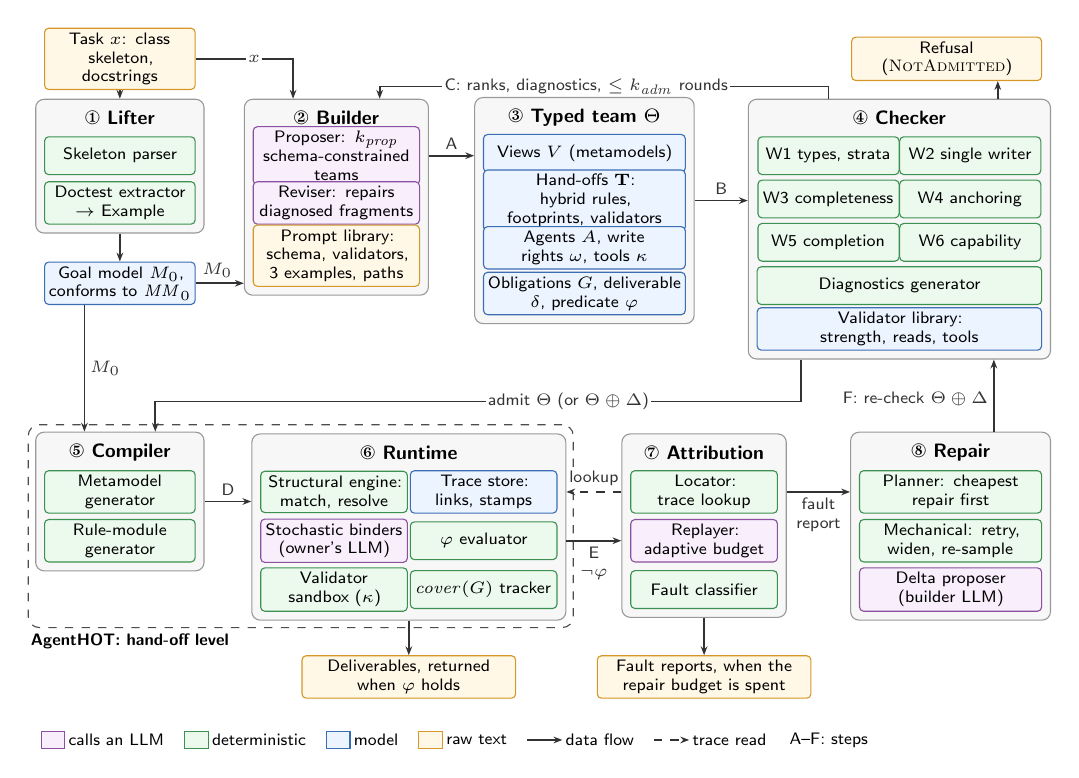
\begin{tikzpicture}[font=\sffamily\scriptsize, >={Stealth[length=3.2pt]}, x=1cm, y=1cm,
  sub/.style={draw, rounded corners=1.5pt, align=center, inner sep=1.6pt, minimum height=4.8mm, text width=#1, font=\sffamily\fontsize{6}{6.8}\selectfont, execute at begin node={\hyphenpenalty=10000\exhyphenpenalty=10000}},
  sub/.default=2.0cm,
  llms/.style={sub=#1, draw=llmbar, fill=llmbg},
  engs/.style={sub=#1, draw=enginebar, fill=enginebg},
  mods/.style={sub=#1, draw=modelbar, fill=modelbg},
  raws/.style={sub=#1, draw=rawbar, fill=rawbg},
  comp/.style={draw=black!40, fill=black!3, rounded corners=3pt, inner sep=3pt},
  ttl/.style={font=\sffamily\scriptsize\bfseries, inner sep=1pt, anchor=center},
  flow/.style={->, semithick, black!80},
  lab/.style={font=\sffamily\fontsize{6}{6.8}\selectfont, fill=white, inner sep=0.8pt, align=center}]

% ================= top row =================
% (1) Lifter
\node[raws=1.8cm] (task) at (1.0,2.3) {Task $x$: class skeleton, docstrings};
\node[ttl] (Lt) at (1.0,1.55) {\ding{172} Lifter};
\node[engs=1.8cm] (sp) at (1.0,1.07) {Skeleton parser};
\node[engs=1.8cm] (ex) at (1.0,0.47) {Doctest extractor $\to$ \cls{Example}};
\node[mods=1.8cm] (goal) at (1.0,-0.55) {Goal model $M_0$, conforms to $\MM_0$};

% (2) Builder
\node[ttl] (Bt) at (3.75,1.55) {\ding{173} Builder};
\node[llms=2.0cm] (prop) at (3.75,1.07) {Proposer: $k_{\mathit{prop}}$ schema-constrained teams};
\node[llms=2.0cm] (rev)  at (3.75,0.47) {Reviser: repairs diagnosed fragments};
\node[raws=2.0cm] (lib) at (3.75,-0.2) {Prompt library: schema, validators, 3 examples, paths};

% (3) Typed team
\node[ttl] (Tt) at (6.9,1.55) {\ding{174} Typed team $\Team$};
\node[mods=2.45cm] (tv) at (6.9,1.1) {Views $V$ (metamodels)};
\node[mods=2.45cm] (tt) at (6.9,0.5) {Hand-offs $\mathbf{T}$: hybrid rules, footprints, validators};
\node[mods=2.45cm] (tw) at (6.9,-0.1) {Agents $A$, write rights $\omega$, tools $\kappa$};
\node[mods=2.45cm] (tg) at (6.9,-0.68) {Obligations $G$, deliverable $\delta$, predicate $\varphi$};

% (4) Checker
\node[ttl] (Ct) at (10.9,1.55) {\ding{175} Checker};
\node[engs=1.68cm] (w1) at (10.0,1.07) {\W{1} types, strata};
\node[engs=1.68cm] (w2) at (11.8,1.07) {\W{2} single writer};
\node[engs=1.68cm] (w3) at (10.0,0.52) {\W{3} completeness};
\node[engs=1.68cm] (w4) at (11.8,0.52) {\W{4} anchoring};
\node[engs=1.68cm] (w5) at (10.0,-0.03) {\W{5} completion};
\node[engs=1.68cm] (w6) at (11.8,-0.03) {\W{6} capability};
\node[engs=3.5cm] (dg) at (10.9,-0.58) {Diagnostics generator};
\node[mods=3.5cm] (vl) at (10.9,-1.13) {Validator library: strength, reads, tools};

\node[raws=2.3cm] (na) at (11.5,2.3) {Refusal (\textsc{NotAdmitted})};

% ================= bottom row =================
% (5) Compiler
\node[ttl] (Kt) at (1.0,-2.7) {\ding{176} Compiler};
\node[engs=1.8cm] (mg) at (1.0,-3.2) {Metamodel generator};
\node[engs=1.8cm] (rg) at (1.0,-3.82) {Rule-module generator};

% (6) Runtime
\node[ttl] (Rt) at (4.67,-2.7) {\ding{177} Runtime};
\node[engs=1.75cm] (se) at (3.72,-3.2) {Structural engine: match, resolve};
\node[mods=1.75cm] (ts) at (5.62,-3.2) {Trace store: links, stamps};
\node[llms=1.75cm] (sb) at (3.72,-3.82) {Stochastic binders (owner's LLM)};
\node[engs=1.75cm] (pe) at (5.62,-3.82) {$\varphi$ evaluator};
\node[engs=1.75cm] (vs) at (3.72,-4.44) {Validator sandbox ($\kappa$)};
\node[engs=1.75cm] (ob) at (5.62,-4.44) {$\mathit{cover}(G)$ tracker};

% (7) Attribution
\node[ttl] (At) at (8.42,-2.7) {\ding{178} Attribution};
\node[engs=1.75cm] (lo) at (8.42,-3.2) {Locator: trace lookup};
\node[llms=1.75cm] (rp) at (8.42,-3.82) {Replayer: adaptive budget};
\node[engs=1.75cm] (cl) at (8.42,-4.44) {Fault classifier};

% (8) Repair
\node[ttl] (Pt) at (11.55,-2.7) {\ding{179} Repair};
\node[engs=2.2cm] (pl) at (11.55,-3.2) {Planner: cheapest repair first};
\node[engs=2.2cm] (mr) at (11.55,-3.82) {Mechanical: retry, widen, re-sample};
\node[llms=2.2cm] (dp) at (11.55,-4.44) {Delta proposer (builder LLM)};

% outputs
\node[raws=2.6cm] (out) at (4.67,-5.55) {Deliverables, returned when $\varphi$ holds};
\node[raws=2.6cm] (fr) at (8.42,-5.55) {Fault reports, when the repair budget is spent};

% ================= containers =================
\begin{scope}[on background layer]
\node[comp, fit=(Lt)(sp)(ex)] (L) {};
\node[comp, fit=(Bt)(prop)(rev)(lib)] (B) {};
\node[comp, fit=(Tt)(tv)(tt)(tw)(tg)] (TH) {};
\node[comp, fit=(Ct)(w1)(w2)(w5)(w6)(dg)(vl)] (C) {};
\node[comp, fit=(Kt)(mg)(rg)] (K) {};
\node[comp, fit=(Rt)(se)(ts)(vs)(ob)] (R) {};
\node[comp, fit=(At)(lo)(rp)(cl)] (AT) {};
\node[comp, fit=(Pt)(pl)(mr)(dp)] (RP) {};
\node[draw=black!70, dashed, rounded corners=4pt, inner sep=2.5pt, fit=(K)(R)] (HOTbox) {};
\end{scope}
\node[anchor=north west, font=\sffamily\fontsize{6.5}{7.5}\selectfont\bfseries, inner sep=1pt] at ([yshift=-1pt]HOTbox.south west) {\tool: hand-off level};

% ================= flows =================
\draw[flow] (task) -- (L.north);
\draw[flow] (L.south) -- (goal.north);
\draw[flow] (task.east) -| node[lab, pos=0.3] {$x$} ([xshift=-0.55cm]B.north);
\draw[flow] (goal.east) -- node[lab, above=1pt, pos=0.45] {$M_0$} (goal.east -| B.west);
\draw[flow] (prop.east -| B.east) -- node[lab, above=1pt] {A} (prop.east -| TH.west);
\draw[flow] (tt.east -| TH.east) -- node[lab, above=1pt] {B} (tt.east -| C.west);
\draw[flow] (C.north) ++(-0.9,0) coordinate (cn) -- (cn |- 0,1.95) -| node[lab, pos=0.27] {C: ranks, diagnostics, $\le k_{\mathit{adm}}$ rounds} ([xshift=0.55cm]B.north);
\draw[flow] (C.north) ++(1.25,0) coordinate (cr) -- (cr |- na.south);
\draw[flow] (C.south) ++(-1.25,0) coordinate (cs) -- (cs |- 0,-2.05) -| node[lab, pos=0.18] {admit $\Team$ (or $\Team\oplus\Delta$)} ([xshift=0.45cm]K.north);
\draw[flow] ([xshift=-0.45cm]goal.south) -- node[lab, right=1pt, pos=0.5] {$M_0$} ([xshift=-0.45cm]goal.south |- K.north);
\draw[flow] (K.east) -- node[lab, above=1pt] {D} (K.east -| R.west);
\draw[flow] (pe.east -| R.east) -- node[lab, below=1pt, align=center] {E\\$\neg\varphi$} (pe.east -| AT.west);
\draw[flow, dashed] (lo.west -| AT.west) -- node[lab, above=1pt] {lookup} (lo.west -| R.east);
\draw[flow] (lo.east -| AT.east) -- node[lab, below=1pt, align=center] {fault\\report} (lo.east -| RP.west);
\draw[flow] (RP.north) ++(0.55,0) coordinate (rn) -- node[lab, pos=0.45, left=1pt] {F: re-check $\Team\oplus\Delta$} (rn |- C.south);
\draw[flow] (R.south) -- (out.north);
\draw[flow] (AT.south) -- (fr.north);

% ================= legend =================
\begin{scope}[every node/.style={font=\sffamily\fontsize{6}{6.8}\selectfont, inner sep=1pt},
  sw/.style={minimum width=3mm, minimum height=2.2mm, inner sep=0}]
\node[sw, draw=llmbar, fill=llmbg] (k1) at (0.15,-6.35) {};
\node[anchor=west] (t1) at (k1.east) {calls an LLM};
\node[sw, draw=enginebar, fill=enginebg, right=6pt of t1] (k2) {};
\node[anchor=west] (t2) at (k2.east) {deterministic};
\node[sw, draw=modelbar, fill=modelbg, right=6pt of t2] (k3) {};
\node[anchor=west] (t3) at (k3.east) {model};
\node[sw, draw=rawbar, fill=rawbg, right=6pt of t3] (k4) {};
\node[anchor=west] (t4) at (k4.east) {raw text};
\coordinate[right=6pt of t4] (l1); \draw[flow] (l1) -- ++(0.45,0) coordinate (l1e);
\node[anchor=west] (t5) at (l1e) {data flow};
\coordinate[right=6pt of t5] (l2); \draw[flow, dashed] (l2) -- ++(0.45,0) coordinate (l2e);
\node[anchor=west] (t6) at (l2e) {trace read};
\node[anchor=west, right=6pt of t6] {A--F: steps};
\end{scope}
\end{tikzpicture}

\caption{Components of \auto{} (\ding{172}--\ding{179}) and their
sub-components. Fill colours give the kind of each sub-component (legend);
grey containers group them into components; the dashed box marks \tool{}, the
hand-off level, and everything else is the team level. Letters A--F mark the steps of
Algorithms~\ref{alg:auto} and~\ref{alg:build}: A~propose candidates, B~check and rank them, C~repair the diagnosed fragments,
D~run, E~attribute a failure, F~re-check a repair delta. No team reaches the
compiler, and no delta reaches the runtime, without passing the checker.}
\label{fig:pipeline}
\end{figure*}

Figure~\ref{fig:pipeline} shows the eight components of \auto{}. The compiler
and the runtime (\ding{176}, \ding{177}) form \tool{}, which executes a typed
team; the other components build, check, diagnose and repair the team.
Table~\ref{tab:mapping} maps each component (second column) to the MDE concept
it reuses (first column). As in
a model-driven tool chain~\cite{bezivin2005unification,brambilla2017mdse},
three kinds of artefact flow between them: \emph{models} that conform to
metamodels (goal model, typed team, trace model, fault reports),
\emph{transformations} (hand-offs and their compiled rule modules) and
\emph{higher-order transformations} that produce or rewrite
transformations~\cite{tisi2009hot}. We follow the running example through the
figure.

\noindent\textbf{\ding{172} Lifter.} Parses the task text (Listing~\ref{lst:task})
into a goal model $M_0$ conforming to the goal view $\MM_0$: a deterministic
text-to-model \emph{injection}~\cite{brambilla2017mdse,bruneliere2014modisco}.

\noindent\textbf{\ding{173} Builder.} The only component that designs. Its
\emph{Proposer} samples up to $k_{\mathit{prop}}$ typed teams, each decoded
under the JSON Schema of a typed team (step~A); the checker ranks them
(step~B). Its \emph{Reviser} repairs the best candidate from its diagnostics
by rewriting only the JSON fragments they name (step~C;
Algorithm~\ref{alg:build}). For \code{TaskBoard} it proposes an Architect, a
Tester and a Developer.

\noindent\textbf{\ding{174} Typed team $\Team$.} The builder's output is a
model, not a set of role prompts: views $V$, hand-offs $\mathbf{T}$ as hybrid
rules with footprints and validators, write rights $\omega$, tools $\kappa$,
goal obligations $G$, a deliverable $\delta$ and an acceptance predicate
$\varphi$ (Definition~\ref{def:typed}), which a program can analyse before it
runs~\cite{cuadrado2017static}.

\noindent\textbf{\ding{175} Checker.} Decides admission by \W{1}--\W{6}
(step~B, Section~\ref{sec:app-check}), with located diagnostics; the number of
diagnostics also ranks the builder's candidates. A team still rejected after
$k_{\mathit{adm}}$ repair rounds is refused (\textsc{NotAdmitted}).

\noindent\textbf{\ding{176} Compiler.} Turns an admitted $\Team$ into
metamodels and rule modules for the runtime (step~D): a \emph{synthesis} higher-order transformation
from the team model to executable transformations, which also loads $M_0$.

\noindent\textbf{\ding{177} Runtime.} Executes hand-offs: the engine fixes
structure, binders ask the owner's LLM for single values, validators check them,
and the $\varphi$ evaluator decides when the run is done
(Section~\ref{sec:app-runtime}).

\noindent\textbf{\ding{178} Attribution} and \textbf{\ding{179} Repair.} When
$\varphi$ fails (step~E), the locator follows trace links to the responsible
binding, the replayer re-samples it and the classifier names the fault
(Section~\ref{sec:app-attr}). The repair planner chooses a mechanical repair
for sampling, footprint and upstream faults and otherwise asks the builder's LLM
for a delta $\Delta$. Every delta, mechanical or not, is an edit operation on
the team model~\cite{kehrer2011lifting,tinnes2025evolution}, and a modification
higher-order transformation~\cite{tisi2009hot} when it changes hand-offs; it
takes effect only after the checker admits $\Team\oplus\Delta$ (step~F).

Algorithm~\ref{alg:auto} gives the same flow as a loop (\textsc{RunTeam}
includes compilation); Algorithm~\ref{alg:build} details steps A--C.

\begin{algorithm}[t]
\caption{\auto{}: build, admit, run, attribute, repair}\label{alg:auto}
\begin{algorithmic}[1]
\Require task $x$; budgets $k_{\mathit{prop}}$, $k_{\mathit{rev}}$, $k_{\mathit{adm}}$ (building), $k_{\mathit{rep}}$ (repair rounds)
\State $M_0\gets\textsc{Lift}(x)$;\ \ $(\Team,\mathit{diag})\gets\textsc{Build}(x,M_0)$ \Comment{Steps A--C, Alg.~\ref{alg:build}}
\If{$\mathit{diag}\neq\emptyset$} \Return \textsc{NotAdmitted}$(\mathit{diag})$ \EndIf
\For{$j=0$ \textbf{to} $k_{\mathit{rep}}$}
  \State $(\varphi,F)\gets\textsc{RunTeam}(\Team,M_0)$ \Comment{Step D: Alg.~\ref{alg:handoff} to fixpoint}
  \If{$\varphi$} \Return \textsc{Done}(deliverables) \EndIf
  \If{$j<k_{\mathit{rep}}$}
    \State $\Delta\gets\textsc{Repair}(\Team,\{\textsc{Attribute}(f)\mid f\in F\})$ \Comment{Step E, Alg.~\ref{alg:attr}}
    \State \textbf{if} $\textsc{Admit}(\Team\oplus\Delta)=\emptyset$ \textbf{then} $\Team\gets\textsc{Apply}(\Team,\Delta)$ \Comment{F; else $\Team$ unchanged}
  \EndIf
\EndFor
\State \Return \textsc{Failed}(fault reports)
\end{algorithmic}
\end{algorithm}

\begin{algorithm}[t]
\caption{\textsc{Build}: proposing and repairing a typed team under the checker (steps A--C)}\label{alg:build}
\begin{algorithmic}[1]
\Require task $x$; goal model $M_0$; budgets $k_{\mathit{prop}}$ (proposals), $k_{\mathit{rev}}$ (repairs per round), $k_{\mathit{adm}}$ (rounds)
\State $\mathcal{C}\gets\emptyset$
\For{$i=1$ \textbf{to} $k_{\mathit{prop}}$} \Comment{Step A, decoded under the typed-team schema}
  \State $\Team_i\gets\textsc{Propose}(x,M_0)$;\ \ $\mathcal{C}\gets\mathcal{C}\cup\{(\Team_i,\textsc{Admit}(\Team_i))\}$ \Comment{Step B, Alg.~\ref{alg:admit}}
  \If{$\textsc{Admit}(\Team_i)=\emptyset$} \textbf{break} \EndIf
\EndFor
\State $(\Team,\mathit{diag})\gets\arg\min_{(\Team',d)\in\mathcal{C}}|d|$ \Comment{the checker ranks the candidates}
\For{$r=1$ \textbf{to} $k_{\mathit{adm}}$ \textbf{while} $\mathit{diag}\neq\emptyset$} \Comment{Step C}
  \State $\Phi\gets\textsc{Fragments}(\Team,\mathit{diag})$;\ \ $P\gets\textsc{Paths}(\Team,\Phi)$ \Comment{named fragments; typed paths}
  \State $\mathcal{R}\gets\{\Team\lhd\textsc{Repair}(\Team,\mathit{diag},\Phi,P)\mid 1..k_{\mathit{rev}}\}$ \Comment{$\lhd$: replace fragments only}
  \If{$\min_{\Team'\in\mathcal{R}}|\textsc{Admit}(\Team')|\ge|\mathit{diag}|$}
    \State $\mathcal{R}\gets\mathcal{R}\cup\{\textsc{Revise}(\Team,\mathit{diag})\}$ \Comment{fallback: whole-team revision}
  \EndIf
  \State $\Team'\gets\arg\min_{\Team''\in\mathcal{R}}|\textsc{Admit}(\Team'')|$
  \If{$|\textsc{Admit}(\Team')|\le|\mathit{diag}|$} $\Team\gets\Team'$;\ \ $\mathit{diag}\gets\textsc{Admit}(\Team')$ \EndIf
\EndFor
\State \Return $(\Team,\mathit{diag})$ \Comment{$\mathit{diag}=\emptyset$ iff $\Team$ is admitted}
\end{algorithmic}
\end{algorithm}

\paragraph{The builder uses the checker} Algorithm~\ref{alg:build} keeps the
division of labour: the LLM proposes and repairs, and only
Algorithm~\ref{alg:admit} admits. It uses the checker in three ways. First,
every proposal and repair is decoded under the JSON Schema of a typed team
(Section~\ref{sec:app-typed}), so a candidate always has the \emph{shape} of a
typed team; whether it is well typed, complete and anchored is still the
checker's decision. Second, because a check costs milliseconds, the builder
samples up to $k_{\mathit{prop}}$ proposals and lets the checker rank them by
their number of diagnostics. Third, the reviser does not regenerate the team:
\textsc{Fragments} maps each diagnostic to the JSON fragments it concerns (a
rule with the classes it creates and reads and its hand-off's sources, a
view, the write rights $\omega$, the agents' tools $\kappa$, the obligations
$G$ and deliverable $\delta$, or $\varphi$; an unanchored goal also offers the
rules and views that should carry it), and \textsc{Paths} lists, for each
diagnosed rule, the navigation paths that type-check from its source variables
(at most two references). The reviser rewrites only these fragments; they are
put back into $\Team$ deterministically ($\lhd$), so a part that was not
diagnosed is never regenerated and a fix cannot be undone by rewriting the
whole team. A whole-team revision is tried only when no localized repair
reduces the number of violations. Section~\ref{sec:res-rq2} measures why this
matters: revising whole teams, a small builder repeats an earlier diagnostic in
almost every round.

% =========================================================================
\subsection{Running an admitted team: hybrid hand-offs}\label{sec:app-runtime}

\paragraph{Views} Every agent owns a \emph{view}, a metamodel that fixes what
it may state (Definition~\ref{def:metamodel}). Views stay heterogeneous; how
they correspond is recorded by trace models (Definition~\ref{def:trace})
rather than by a shared schema, as in view-based
development~\cite{klare2021vitruvius,bruneliere2019views}. One view is special:
the \emph{goal view} $\MM_0$, into which the task is lifted. In the running
example, \textsc{Lift} parses the class skeleton of Listing~\ref{lst:task}
deterministically into a goal model $M_0$ with one \cls{Task}, three
\cls{Method}s and three \cls{Example}s (Listing~\ref{lst:views}); doctests are
moved out of \code{docstring} into \cls{Example} objects, so a rule that reads
a docstring does not see the examples.

\begin{lstlisting}[float=tb, language=KM3, style=model, caption={Goal view and agent views of the typed \devteam{} in KM3 notation~\cite{jouault2006km3}; \code{Goal.Method} is an external (cross-view) reference.}, label={lst:views}]
package Goal {                                                   -- MM0, filled by Lift
  class Task       { attribute name : String;  attribute description : String;
                     reference methods [1-*] container : Method;
                     reference examples [0-*] : Example; }       -- in docstring order
  class Method     { attribute name : String;  attribute signature : String;
                     attribute docstring : String;  reference task : Task;
                     reference examples [0-*] container : Example; }
  class Example    { attribute call : String;  attribute expected : String; } }
package Design { class MethodDesign { attribute name : String;  attribute contract : String;
                                      reference method : Goal.Method; } }
package Test   { class TestCase     { attribute name : String;  attribute code : String;
                                      reference method : Goal.Method; } }
package Code   { class MethodImpl   { attribute name : String;  attribute body : String;
                                      reference method : Goal.Method; } }
\end{lstlisting}

\paragraph{Hybrid hand-offs} A hand-off is written as matched rules
(Definition~\ref{def:rule}). \tool{} splits every rule along the line that
ATL's two-phase execution already draws: matching, object creation and
reference resolution stay with a deterministic engine, and only bindings whose
value no OCL expression can compute go to an LLM. Two design choices follow from
the aim of making failures diagnosable. Each LLM call sees a declared
\emph{footprint} rather than the whole conversation, so that what a value was
produced from is recorded and can be replayed; and LLM-written values never
steer structure (stratification, below), so that which objects exist is a
deterministic function of the goal.

\begin{definition}[Hybrid rule, stochastic binding, footprint, owner]\label{def:hybrid}
A hybrid rule is a matched rule whose bindings are partitioned as
$B_r=B_r^{\mathrm{str}}\uplus B_r^{\mathrm{sem}}$. A \emph{structural} binding
$f\leftarrow e$ is evaluated by the engine. A \emph{stochastic} binding
$b=f\leftarrow\texttt{@llm}(\pi_b,\,e_b)\ \texttt{@check}\ \chk_b$ targets a
primitive attribute $f$; its OCL expression $e_b$ defines the \emph{footprint}
$\fp_b(m)$ of a match $m$, the set of source locations (object, feature) whose
values the LLM may see; $\pi_b$ is a prompt; and $\chk_b$ is a \emph{validator},
a predicate over the candidate value and a declared set of \emph{validator
reads} $\mathit{vr}_b(m)$. The \emph{owners} of a hand-off $T$ are the agents
whose write rights $\omega$ (Definition~\ref{def:typed}) include its target view,
$\mathit{owner}(T)=\{a\mid\mathit{tgt}(T)\in\omega(a)\}$, a singleton by \W{2}; a binding's owners are those of
its hand-off. The \emph{version stamp} of an accepted value is a digest
$\#(\fp_b(m)\cup\mathit{vr}_b(m))$ of the \emph{values} at all locations its
production and its check read.
\end{definition}

\begin{definition}[Semantics of a hybrid hand-off]\label{def:hsem}
Let the \emph{structural part} $T^{\mathrm{str}}$ of a hybrid hand-off $T$ be
$T$ with every stochastic binding removed. Given source models $\vec M$,
$T^{\mathrm{str}}(\vec M)$ is computed by ATL's matching and initialisation and
is a deterministic \emph{skeleton}. Like a relation of QVT Relations
(QVT-R)~\cite{omg2016qvt,stevens2010qvt},
and unlike an ATL function, the hand-off denotes the \emph{set} of
admissible targets
\[\llbracket T\rrbracket(\vec M)=\{M_t\mid M_t\sqsupseteq T^{\mathrm{str}}(\vec M)\ \wedge\ \forall(m,b):\ \chk_b(M_t[m,b],\mathit{vr}_b(m))\},\]
where $M_t\sqsupseteq T^{\mathrm{str}}(\vec M)$ means that $M_t$ extends the
skeleton by exactly one value $M_t[m,b]$ per match $m$ and stochastic binding $b$.
We require $\mathit{tgt}(T)\notin\mathit{src}(T)$. An execution samples one
element of this set, or \emph{escalates} the bindings for which no admissible
value was found; an escalated execution lies outside $\llbracket T\rrbracket$
and makes the run fail. A team denotes the set of tuples of models, one per
view, in which every hand-off's target is admissible for its sources; on the
acyclic hand-off graph these are obtained hand-off by hand-off in topological
order. The footprint does not appear in $\llbracket T\rrbracket$: it is an
information-flow constraint on how a value is produced, enforced by the
runtime (Algorithm~\ref{alg:handoff}).
\end{definition}

The skeleton is deterministic only if it does not depend on values that an LLM
wrote. We therefore require \emph{stratification}: no guard and no structural
binding may read a feature written by a stochastic binding. This is checked by
\W{1} (Section~\ref{sec:app-check}). Our runtime departs from ATL in two
deliberate ways. First, a reference binding whose expected type lies in a
\emph{source} view (for example \code{method <- m}, typed \code{Goal.Method})
creates a cross-view link to the source object instead of being resolved
through the trace, because agents' views refer to the goal by design. ATL would resolve \code{m} to the target that
\code{m}'s own rule created, which here has the wrong type; we apply that
resolution only to references whose type lies in the \emph{target} view.
Second, trace models are persisted, as in MeTAGeM-Trace~\cite{vara2014metagem}.

\begin{lstlisting}[float=tb, language=ATL, style=model, caption={The three hybrid hand-offs of the admitted typed \devteam{}. \code{@llm} marks a stochastic binding (second argument: footprint); \code{@check} its validator.}, label={lst:rules}]
rule Method2Design {                             -- Goal -> Design (owner: Architect)
  from m : Goal!Method
  to   d : Design!MethodDesign ( name <- m.name, method <- m,
         contract <- @llm('State a contract', Sequence{m.name, m.signature, m.docstring})
         @check nonempty(contract) ) }
rule Method2Test {                               -- Goal -> Test (owner: Tester)
  from m : Goal!Method
  to   t : Test!TestCase ( name <- m.name, method <- m,       -- structural; cross-view link
         code <- @llm('Write unit tests for this method',
                      Sequence{m.signature, m.docstring, m.examples.call, m.examples.expected})
         @check test_valid(code, m) ) }                        -- behaviour validator
rule Design2Impl {                               -- Design, Test -> Code (owner: Developer)
  from d : Design!MethodDesign, t : Test!TestCase (t.method = d.method)
  to   i : Code!MethodImpl ( name <- d.name, method <- d.method,
         body <- @llm('Implement the method',
                      Sequence{d.method.signature, d.contract, t.code})
         @check compiles(body) and passes_tests(body, t.code) ) }
\end{lstlisting}

In \code{Method2Test} (Listing~\ref{lst:rules}), which test cases exist and which method each belongs to
is decided by the engine; the LLM writes only the code, from that method's
signature, docstring and examples, so no LLM can forget to test
\code{mark\_done}.

\begin{algorithm}[t]
\caption{\tool{}: executing one hybrid hand-off $T$ (runtime)}\label{alg:handoff}
\begin{algorithmic}[1]
\Require hand-off $T$; sources $\vec{M}$; target $M_t$; trace model $\TL_T$; budget $k$
\State compute $T^{\mathrm{str}}(\vec M)$ incrementally; update $M_t$ and $\TL_T$ \Comment{structure only}
\For{each stochastic binding $(t,b)$ of a match $m$ whose stamp is stale}
  \For{$i=1$ \textbf{to} $k$}
    \State $v\gets\textsc{LLM}_{\mathit{owner}(T)}(\pi_b,\fp_b(m))$ \Comment{the prompt contains the footprint only}
    \If{$\chk_b(v,\mathit{vr}_b(m))$} accept $v$; update $\mathit{stamp}(t,b)$; \textbf{break} \EndIf
  \EndFor
  \If{no value was accepted} $\mathit{Esc}\gets\mathit{Esc}\cup\{(t,b)\}$ \Comment{escalate} \EndIf
\EndFor
\State \Return $M_t,\TL_T,\mathit{Esc}$
\end{algorithmic}
\end{algorithm}

\paragraph{Agents at run time} An agent is a role prompt, a model and a set of
tools $\kappa(a)$. Agents do not converse. Each stochastic binding is one LLM
call of its owner whose prompt is the role prompt, $\pi_b$ and the footprint
serialised as a list of \emph{object.feature = value} lines; production uses no
tools. Tools are used by validators, which run in a sandbox that grants exactly
$\kappa(a)$ of the owner. Agents therefore see each other's work only through
footprints, which is what makes a recorded footprint sufficient for replay.

\paragraph{Execution and change} Algorithm~\ref{alg:handoff} executes one
hand-off: line~1 is ATL's matching and initialisation, made
incremental~\cite{jouault2010incremental}; lines~2--6 sample only values whose
stamp is missing or \emph{stale} (differs from $\#(\fp_b(m)\cup\mathit{vr}_b(m))$), prompt with the footprint only, and escalate after
$k$ rejections. The runtime repeats it over all hand-offs in topological order
until no model changes. A change $\Delta$ that modifies the locations
$\mathit{loc}(\Delta)$ yields the \emph{stale set} $\Obl(\Delta)$, the least
set of pairs $(t,b)$, over the trace models of all hand-offs, such that
$\fp_b(m)\cup\mathit{vr}_b(m)$ meets $\mathit{loc}(\Delta)$ or a location
written by a pair already in $\Obl(\Delta)$: the values whose stamps become
stale, directly or transitively. If E2.2 is changed to expect \code{KeyError},
the stale set contains the test code of \code{mark\_done} and, one hop later, its
implementation; other values keep their stamps, so re-establishing $\varphi$
costs at most $k\cdot|\Obl(\Delta)|$ LLM calls. This is an analytical property
of the runtime; we use it for repair (Section~\ref{sec:app-attr}) but do not
evaluate arbitrary source changes in this paper.

\paragraph{Implementation} The compiler and runtime are written in Python.
Models are JSON object graphs validated against a JSON Schema generated from
each view; rule modules are data interpreted by the engine; guards, bindings
and footprints use an OCL fragment of navigation paths, literals, comparisons
and conjunction. The deliverable $\delta=(D,g)$ names a target class and
feature (\code{MethodImpl.body}); the runtime assembles the deliverable by
inserting every $g$ value into the class outline given by $M_0$ (for
function-level tasks, into the function signature).
Behaviour validators run on that assembled artefact, with methods that have no
accepted value yet replaced by stubs, and examples run in docstring order on
one object, as doctest does, so E2.1 can rely on the task added by E1.1.

\begin{definition}[Run record, descendants, acceptance]\label{def:accept}
At run time every trace link $(m,t,r)$ carries, for each stochastic binding $b$
of $r$, a record $(b,\fp_b(m),\mathit{vr}_b(m),\mathit{stamp},v)$ with the
accepted value $v$ or an escalation mark. The link \emph{connects} to each
object in $t$ every object of $m$ and every object owning a location in a
recorded footprint or validator read. An object $o'$ is a \emph{descendant} of
$o$ if a chain of connections leads from $o$ to $o'$. Then
$\varphi$ contains the engine clauses $\mathit{cover}(G)$, $\mathit{valid}$,
$\mathit{fresh}$ and $\mathit{noEsc}$, and may add library clauses (\W{5}),
where $\mathit{cover}(G)$ holds if every goal object $o$ in the scope of an
obligation $(C,s,\mu,F_C)$ has a descendant holding an accepted value of a
behaviour-validated binding ($\mu=\mathit{checked}$) or of the deliverable
feature ($\mu=\mathit{delivered}$); $\mathit{valid}$ if every accepted value
passes its validator on the final models; $\mathit{fresh}$ if every stamp
equals the digest of the current values; and $\mathit{noEsc}$ if nothing is
escalated. $\mathit{cover}(G)$ is deliberately one-sided; that producer and
check both read the goal is ensured statically by \W{4}.
\end{definition}

An \cls{Example} thus has as descendant the test case whose footprint read it,
although no rule matches \cls{Example}. The engine, not an agent, decides that
the team is done; a Tester that declares success early cannot end the run while
the test for E2.2 fails. An escalation is a recorded fault, not a hand-over to
a person: it makes $\mathit{noEsc}$ false and becomes input to attribution.

% =========================================================================
\subsection{What the builder proposes: typed teams}\label{sec:app-typed}

\tool{} executes a team but does not design one. In \auto{} a builder LLM
writes the views, rules and validators, so they become an artefact that must
be checked. A free-form builder outputs role prompts (Listing~\ref{lst:freeteam});
an \auto{} builder must output a \emph{typed team}.

\begin{definition}[Typed team]\label{def:typed}
A typed team is a tuple $\Team=(A,V,\mathbf{T},\omega,\kappa,G,\delta,\varphi)$ where
$A$ is a set of agents, each with a free-text role prompt; $V=\{\MM_0,\dots,\MM_n\}$
a set of views with goal view $\MM_0$; $\mathbf{T}$ a set of hybrid hand-offs,
each with source views $\mathit{src}(T)\subseteq V$ and one target view
$\mathit{tgt}(T)\neq\MM_0$; $\omega:A\to2^V$ the write rights;
$\kappa:A\to2^{\mathit{Tools}}$ the tools of each agent; $G$ a set of
\emph{goal obligations} $(C,s,\mu,F_C)$ of a goal class $C$, a scope predicate
$s$, a mode $\mu\in\{\mathit{checked},\mathit{delivered}\}$ and a set of
\emph{anchor features} $F_C$ of $C$ (by default, all attributes of $C$);
$\delta=(D,g)$ the \emph{deliverable feature}; and $\varphi$ the proposed
acceptance predicate, a conjunction of the four engine clauses of
Definition~\ref{def:accept} and optional library clauses (\W{5}). $\MM_0$ and $M_0$ are
produced by \textsc{Lift}; the builder cannot change them.
\end{definition}

The tools that a stochastic binding needs, $\tau(b)$, are not proposed: they are
derived from the validator library. To keep every condition decidable, the
builder fills a JSON format whose JSON Schema plays the role of the typed-team
metamodel (and constrains the builder's decoding, Algorithm~\ref{alg:build}), in which guards are
conjunctions of comparisons between navigation paths and literals, structural
bindings and footprints are navigation paths or literals, and validators are
chosen from a library. Each library entry declares a \emph{strength}
(\emph{form}: parses, compiles, conforms; \emph{behaviour}: executes the value
against an oracle or test), the tools it needs, and which of its arguments it
\emph{reads}; Table~\ref{tab:validators} lists the entries used in this paper.
An obligation of mode \emph{checked} requires that the goal's anchor features
reach a behavioural check; one of mode \emph{delivered} requires a deliverable
for every in-scope goal object.

\begin{table}[t]
\centering\scriptsize
\caption{Validator library entries used in the examples and the evaluation.
Reads: features the validator inspects besides the candidate value.}
\label{tab:validators}
\setlength{\tabcolsep}{3pt}
\begin{tabularx}{\textwidth}{@{}l l >{\raggedright\arraybackslash}X >{\raggedright\arraybackslash}p{2.3cm} l@{}}
\toprule
Validator & Strength & Accepts the candidate value $v$ if & Reads & Tools \\
\midrule
\code{nonempty(v)} & form & $v$ is a non-empty string & -- & -- \\
\code{compiles(v)} & form & $v$ parses and compiles as Python & -- & -- \\
\code{smoke\_test(v, b)} & behaviour & $v$ is the outcome of a fixed smoke test of the class assembled with body $b$ & $b$ & \code{exec} \\
\code{test\_valid(v, m)} & behaviour & $v$ runs, fails on a stub of $m$, and asserts every example of $m$ & \code{m.signature}, \code{m.examples.*} & \code{exec} \\
\code{passes\_tests(v, c)} & behaviour & the assembled class with $v$ passes the test code $c$ & $c$ & \code{exec} \\
\code{examples\_run(v, m)} & behaviour & the assembled class with $v$ passes the examples of $m$ & \code{m.examples.*} & \code{exec} \\
\bottomrule
\end{tabularx}
\end{table}

\begin{lstlisting}[float=tb, style=model, caption={An illustrative first proposal of a typed \devteam{}, rendered from JSON. It contains one instance of each defect \D{1}--\D{5}.}, label={lst:proposal}]
agents:   Architect{tools: []}  Tester{tools: []}  Developer{tools: [exec]}            -- D5
writes:   Architect: Design     Tester: Test       Developer: Code, Test                -- D3
goal:     (Example, all, checked, {call, expected})   (Method, all, delivered)
deliver:  MethodImpl.body
handoffs:
  Method2Design : Goal -> Design
      contract <- @llm(.., Sequence{m.name, m.signature})        @check nonempty
  Design2Impl   : Design -> Code
      body     <- @llm(.., Sequence{d.contract, d.returnType})   @check compiles         -- D2
  Impl2Run      : Code -> Test
      verdict  <- @llm('Run and judge', i.body)          @check smoke_test(verdict, i.body)
done:     cover(G), valid, fresh, noEsc, Tester.says('ALL TESTS PASS')                  -- D4
\end{lstlisting}

Listing~\ref{lst:proposal} reads well: an Architect designs, a Developer
implements, a Tester runs the code. Yet no rule reads an \cls{Example}, so E2.2
cannot influence anything that is checked (\D{1}); the Developer's prompt refers
to \code{d.returnType}, which the Design view does not declare (\D{2});
Developer and Tester both write the Test view (\D{3}); completion includes a
claim by the Tester (\D{4}); and the Tester must run code without the tool to do
so (\D{5}).

% =========================================================================
\subsection{Admission: six well-formedness conditions}\label{sec:app-check}

The checker evaluates six conditions on the typed team alone: no task data, no
LLM call and no execution. \W{1}--\W{3} adapt to LLM-authored teams checks that
static analysers perform on hand-written ATL
transformations~\cite{cuadrado2017static}; \W{4}--\W{6} concern the team as a
whole. Two graphs support them. The \emph{hand-off graph} has an edge
$\MM_i\to\MM_j$ for every hand-off with $\MM_i\in\mathit{src}(T)$ and
$\MM_j=\mathit{tgt}(T)$. The data-flow graph works on features.

\begin{definition}[Feature-level data flow]\label{def:dataflow}
$\mathcal{F}_\Team$ has a node $(C,f)$ for every class $C$ and feature $f$ of
every view. A binding that writes feature $g$ of class $D$ contributes a
\emph{production} edge $(C,f)\to_p(D,g)$ for every $(C,f)$ that its expression
or footprint reads, and a \emph{check} edge $(C,f)\to_c(D,g)$ for every $(C,f)$
that its validator reads. A navigation path such as \code{m.examples.call} reads
\code{Method.examples} and \code{Example.call}. Let $\mathcal{B}$ be the
features written by stochastic bindings whose validator has behavioural
strength. A goal obligation $(C,s,\mathit{checked},F_C)$ is \emph{anchored} at
$(D,g)\in\mathcal{B}$ if every anchor feature in $F_C$ reaches $(D,g)$ along a
path of production edges, \emph{and} every anchor feature reaches $(D,g)$ along
a path of production edges followed by one check edge. (Goal data flows only
along production edges; a check edge gates acceptance but transmits nothing.)
\end{definition}

Anchoring is two-sided on purpose: the producer of the checked value must have
seen the goal, and its check must test against the goal. Section~\ref{sec:res-rq2}
shows that the one-sided variant (check edges alone suffice) admits teams whose
producers never see the goal.

\paragraph{\W{1} Hand-offs are well typed and stratified} Every rule reads
only its source views and writes only features its target class declares; every
guard, binding and footprint path type-checks; stochastic bindings target
primitive attributes and use a library validator with correctly typed
arguments; and no guard or structural binding reads a feature written by a
stochastic binding. \emph{Rules out the formal part of \D{2}.}

\paragraph{\W{2} Every artefact has one writer} The write rights $\omega(a)$
are pairwise disjoint and cover $V\setminus\{\MM_0\}$, so
$\mathit{owner}(T)$ is a single agent; and every class is created by at most
one rule, so no object has two producers.
\emph{Rules out \D{3}.} The condition is conservative: rules with provably
disjoint guards could share a target class.

\paragraph{\W{3} Targets are complete} Every mandatory feature of a created
class is bound exactly once; every reference binding whose type lies in the
target view is \emph{resolvable} (some rule maps the yielded source class to
the expected class); and every reference whose type lies in a source view
yields objects of that type. A guard that equates two such structural
references to the same goal object is a \emph{join} (as \code{t.method =
d.method}). \emph{Rules out the content part of \D{2}.}

\paragraph{\W{4} Every goal is anchored} (a) Every obligation of mode
\emph{checked} is anchored at some feature of $\mathcal{B}$
(Definition~\ref{def:dataflow}), and every source-pattern class of a rule on
the anchoring chain is \emph{total}: a goal class, or a class created by a rule
whose guard is implied by the scope; every obligation of mode \emph{delivered} reaches $\delta$ along
production edges. (b) Every view is reachable from
$\MM_0$ in the hand-off graph and reaches a view that contains a feature of
$\mathcal{B}$: there is no idle or unverified agent. \emph{Rules out \D{1}.}

\paragraph{\W{5} The engine decides completion} $\varphi$ consists of engine
clauses only (from the vocabulary
$\{\mathit{cover}(G),\mathit{valid},\mathit{fresh},\mathit{noEsc}\}$, all four
required, plus optional library clauses such as running the public examples on
the deliverable), and the hand-off graph is acyclic. \emph{Rules out \D{4}.}
Builders may add clauses; \W{5} rejects any clause that is a claim by an
agent.

\paragraph{\W{6} Work goes to agents that can do it} For every stochastic
binding $b$, $\tau(b)\subseteq\kappa(\mathit{owner}(b))$. In \tool{}, an owner's
validators run in the owner's sandbox, whose capabilities are exactly
$\kappa(a)$; production itself uses no tools. An agent without \code{exec} therefore cannot run the oracle that decides whether
its value is accepted, just as a Gaia role cannot act outside its
permissions~\cite{wooldridge2000gaia}. \emph{Rules out \D{5}.}

\begin{algorithm}[t]
\caption{\textsc{Admit}: deciding whether a typed team $\Team$ may run}\label{alg:admit}
\begin{algorithmic}[1]
\Require typed team $\Team=(A,V,\mathbf{T},\omega,\kappa,G,\delta,\varphi)$; validator library
\State $\mathit{diag}\gets\textsc{TypeCheck}(\mathbf{T},V)\cup\textsc{Stratification}(\mathbf{T})$ \Comment{\W{1}}
\State $\mathit{diag}\gets\mathit{diag}\cup\textsc{Writers}(\omega,\mathbf{T})\cup\textsc{Completeness}(\mathbf{T})$ \Comment{\W{2}, \W{3}}
\State build $\mathcal{F}_\Team$ with production and check edges; $\mathcal{B}\gets$ behaviour-checked features
\For{each $(C,s,\mu,F_C)\in G$ that is not anchored (or, if delivered, does not reach $\delta$)}
  \State $\mathit{diag}\gets\mathit{diag}\cup\{(\W{4},C)\}$ \Comment{\W{4}(a)}
\EndFor
\State $\mathit{diag}\gets\mathit{diag}\cup\{(\W{4},V')\mid V'\text{ unreachable from }\MM_0\text{ or not reaching }\mathcal{B}\}$ \Comment{\W{4}(b)}
\State $\mathit{diag}\gets\mathit{diag}\cup\textsc{EngineClauses}(\varphi)\cup\textsc{Cycles}(\mathbf{T})$ \Comment{\W{5}}
\State $\mathit{diag}\gets\mathit{diag}\cup\{(\W{6},b)\mid\tau(b)\not\subseteq\kappa(a),\ a\text{ writes }\mathit{tgt}(b)\}$ \Comment{\W{6}}
\State \Return $\mathit{diag}$ \Comment{empty iff $\Team$ is admitted}
\end{algorithmic}
\end{algorithm}

Algorithm~\ref{alg:admit} returns diagnostics that name the condition, the
offending element and a hint. When \W{2} fails, \W{6} is evaluated for every
agent that writes the target view. Listing~\ref{lst:diag} is the output of our
checker on Listing~\ref{lst:proposal}: one violation per seeded defect and no
other. Unlike an LLM critic's comments, diagnostics are \emph{complete} for the
conditions checked and name a rule, path or write right rather than ``improve
coordination''.

\begin{lstlisting}[float=tb, style=engine, caption={Checker output on Listing~\ref{lst:proposal}.}, label={lst:diag}]
W1  Design2Impl.body: footprint path 'd.returnType':
        Design!MethodDesign has no feature 'returnType'
W2  view Test written by ['Developer', 'Tester']; needs exactly one writer
W4  goal (Example, all, checked): anchor features {call, expected}
        reach no behaviour-checked value
W5  done-clause Tester.says('ALL TESTS PASS') is not an engine clause
W6  Impl2Run.verdict needs ['exec']; writer Tester has []
REJECTED: 5 violation(s)
\end{lstlisting}

\paragraph{Why anchoring} A class-level path is not enough: a builder can
create one test case per method written from the method's \emph{name} only, so
a path from \cls{Method} to a checked class exists, yet no example ever
influences a check. Figure~\ref{fig:w4} computes \W{4} for the admitted team,
where \code{Example.call} reaches \code{TestCase.code} by a production and a
check edge, and for the first proposal, where no edge leaves \cls{Example}.

\begin{figure}[t]
\centering
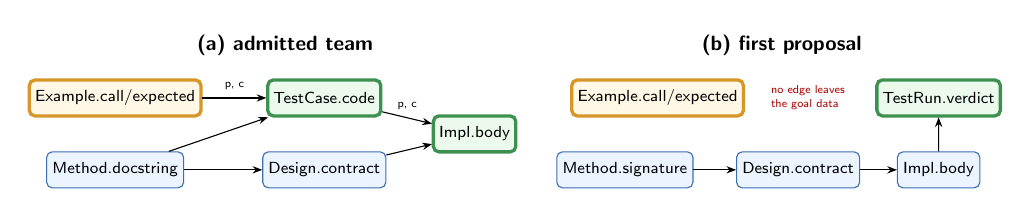
\begin{tikzpicture}[scale=0.83, transform shape, font=\sffamily\scriptsize, >={Stealth[length=3.5pt]},
  f/.style={draw=modelbar, fill=modelbg, rounded corners=2pt, minimum height=5.5mm, inner sep=2.5pt},
  b/.style={draw=enginebar, fill=enginebg, rounded corners=2pt, minimum height=5.5mm, inner sep=2.5pt, very thick},
  g/.style={draw=rawbar, fill=rawbg, rounded corners=2pt, minimum height=5.5mm, inner sep=2.5pt, very thick}]
  \node[font=\sffamily\small\bfseries] at (2.6,1.15) {(a) admitted team};
  \node[g] (ex) at (0,0.35) {Example.call/expected};
  \node[f] (doc) at (0,-0.75) {Method.docstring};
  \node[b] (tc) at (3.2,0.35) {TestCase.code};
  \node[f] (con) at (3.2,-0.75) {Design.contract};
  \node[b] (body) at (5.5,-0.2) {Impl.body};
  \draw[->] (ex) -- node[above, font=\sffamily\tiny] {p, c} (tc); \draw[->] (doc) -- (tc); \draw[->] (doc) -- (con);
  \draw[->] (con) -- (body); \draw[->] (tc) -- node[above, font=\sffamily\tiny] {p, c} (body);
  \node[font=\sffamily\small\bfseries] at (10.2,1.15) {(b) first proposal};
  \node[g] (ex2) at (8.3,0.35) {Example.call/expected};
  \node[f] (sig2) at (7.8,-0.75) {Method.signature};
  \node[f] (con2) at (10.45,-0.75) {Design.contract};
  \node[f] (body2) at (12.6,-0.75) {Impl.body};
  \node[b] (ver2) at (12.6,0.35) {TestRun.verdict};
  \draw[->] (sig2) -- (con2); \draw[->] (con2) -- (body2); \draw[->] (body2) -- (ver2);
  \node[text=red!65!black, align=left, font=\sffamily\tiny] at (10.6,0.35) {no edge leaves\\the goal data};
\end{tikzpicture}
\caption{Feature-level data flow for \W{4}. Yellow: anchor features of the
obligation $(\cls{Example},\mathit{all},\mathit{checked})$. Green: behaviour-checked
features. ``p, c'': the edge exists both as a production and as a check edge.
(a) is anchored; in (b) nothing reads an \cls{Example}, so \W{4} fails although
the team does test \emph{something}.}
\label{fig:w4}
\end{figure}

\paragraph{Limits} Whether a guard excludes in-scope objects is undecidable in
general; the checker accepts guards implied by the obligation's scope, warns
about others, and $\mathit{cover}(G)$ enforces coverage at run time. An
undeclared obligation is not checked.

\begin{proposition}[Cost]\label{prop:cost}
\W{1}--\W{6} are decidable on $\Team$ in time polynomial in $|\Team|$
(classes, features, rules, bindings and path segments).
\end{proposition}
\begin{proof}[Sketch]
\W{1} navigates each path once; \W{2}, \W{3} and \W{6} compare finite sets;
\W{4} is reachability over production edges, extended by one check edge, in
$\mathcal{F}_\Team$, whose size is bounded by path segments times bindings;
\W{4}(b) and the cycle test of \W{5} are searches on the hand-off graph.
\end{proof}

\begin{proposition}[Structural coverage]\label{prop:struct}
Let $\Team$ be admitted, and let every guard on the rule chains that anchor an
obligation $(C,s,\mathit{checked},F_C)$ either be implied by $s$ or equate
structural references to the same goal object (a join, \W{3}). Then, for every
object $o$ of class $C$ that satisfies $s$, the skeletons
$T^{\mathrm{str}}$ create a chain of descendants of $o$ that ends in a target
object $t$ with a behaviour-checked feature whose footprint and validator reads
both contain data derived from $o$. Consequently, if $\mathit{cover}(G)$ fails
for $o$ at the end of a run, some stochastic binding on that chain is escalated
or invalid.
\end{proposition}
\begin{proof}[Sketch]
By \W{1}, skeletons do not depend on LLM-written values, so matches depend only
on goal data and on objects created by earlier skeletons. Induction along the
anchoring path of Definition~\ref{def:dataflow}: each production edge stems
from a rule whose source pattern contains the class of its tail or an object
from which its footprint navigates to the tail (as \code{m.examples.call});
that object exists by induction, the other source-pattern variables are filled
because their classes are total (\W{4}), a guard implied by $s$ holds, and a join holds
because both joined objects exist and were linked to the same goal object by
structural bindings; so the rule fires and, by \W{3}, creates its target with
all mandatory features. Hence every object on the chain exists
and only stochastic values can be missing; a missing or rejected one is, by
Algorithm~\ref{alg:handoff}, escalated or reported by $\mathit{valid}$.
\end{proof}

Proposition~\ref{prop:struct} turns attribution into a lookup: a coverage
failure is never a silent structural gap but points at a named binding.
Admission does \emph{not} guarantee that the views capture what the task needs,
that validators are strong enough, or that agents reason well.

% =========================================================================
\subsection{Attribution and checked repair}\label{sec:app-attr}

\paragraph{Locate} If $\varphi$ fails, the engine knows which clauses fail
and, through the trace models, where. A failed $\mathit{valid}$ clause or an
escalation names one pair $(t,b)$: a target object, a stochastic binding, its
rule, hand-off and owner, and the stamped footprint its LLM saw. A failed
$\mathit{cover}(G)$ clause, by Proposition~\ref{prop:struct}, names a binding
on the anchoring chain. Locating the \emph{symptom} is therefore a lookup, not
an inference over a transcript. This exploits the observation that attribution
needs the \emph{input} of each step~\cite{chen2026traceelephant}, which in
\tool{} is a declared, bounded footprint.

\paragraph{Classify} The symptom's binding is not always the cause.
Algorithm~\ref{alg:attr} replays the binding on its recorded footprint to
decide why it failed.

\begin{algorithm}[t]
\caption{\textsc{Attribute}: classifying a failed stochastic binding $(t,b)$}\label{alg:attr}
\begin{algorithmic}[1]
\Require failed value $v$ of $b$; recorded footprint $\phi$; replay cap $n_{\mathit{rep}}$; hop limit $h$
\If{$\chk_b(v,\mathit{vr}_b)$ is unstable over reruns} \Return \textsc{Validator} \EndIf
\If{\textsc{Replays}$(b,\phi)$ pass sometimes} \Return \textsc{Sampling} \EndIf
\For{$j=1$ \textbf{to} $h$}
  \If{\textsc{Replays}$(b,\phi\cup\textsc{Widen}_j(\phi))$ pass sometimes} \Return \textsc{Footprint}$(j)$ \EndIf
\EndFor
\For{each value $u\in\phi$ written upstream by a stochastic binding $b'$}
  \If{re-sampled $u$ makes \textsc{Replays}$(b,\phi)$ pass} \Return \textsc{Upstream}$(b')$ \EndIf
\EndFor
\State \Return \textsc{Specification} \Comment{no supported value satisfies $\chk_b$}
\end{algorithmic}
\end{algorithm}

\textsc{Widen}$_j$ adds every path from the rule's source variables that follows
at most $j$ references and ends in an attribute; a footprint repair keeps only
the added paths without which no replay passes. \textsc{Replays} draws samples
one at a time and, in the \emph{adaptive} budget, stops at the first pass
(``passes sometimes''); if none of $n_{\mathit{rep}}=3$ samples passes, it
does not. We use hop limit $h=2$. The stability test of line~1 reruns the
validator three times, which costs no LLM call. An \textsc{Upstream}$(b')$
result is followed by attributing $b'$ with its accepted value treated as
failed.
A \emph{validator} fault blames the check; a \emph{sampling} fault means the
composition was adequate and the owner's LLM unlucky or weak (retry, or use a
stronger model); a \emph{footprint} fault is an instance of \D{2} (widen the
footprint by the paths that made the replay pass); an \emph{upstream} fault
moves responsibility to the producer of an input; a \emph{specification} fault
means no value the footprint supports satisfies the prompt and validator. The
procedure makes at most $(h+1+|\mathit{up}(b)|)\,n_{\mathit{rep}}+|\mathit{up}(b)|$
LLM calls per binding visited (plus the replays that minimise a footprint
repair), where $\mathit{up}(b)$ are the upstream
stochastic values in its footprint, and visits at most as many bindings as the longest path in the hand-off graph.

\paragraph{Checked repair} A fault report becomes a team delta $\Delta$:
mechanically for sampling, footprint and upstream faults (retry, widen,
re-sample), and by the builder otherwise. $\Team\oplus\Delta$ is the typed team
with $\Delta$'s edits applied; the checker evaluates it with
Algorithm~\ref{alg:admit}, and only if it is admitted does \textsc{Apply}
install it in the running team, as described next. Every delta is an edit of the team model, and a modification
higher-order transformation~\cite{tisi2009hot} when it changes hand-offs; as
for consistency-preserving operators~\cite{horcas2023consistency,alomar2021preserving},
deltas differ in what they preserve. A delta that changes only rules, prompts, footprints or
validators is applied \emph{in place}: affected values lose their stamps and
become stale, and all other accepted values are kept. A delta that only
adds views, agents or hand-offs is applied \emph{by extension}: the compiler
generates the new rule modules, so that new agents receive work for everything
already built. Any other delta \emph{rebuilds} the team, as a free-form builder
must always do. The runtime is regenerated from the team model, one way.

\paragraph{Running example, end to end} The first proposal
(Listing~\ref{lst:proposal}) is rejected with five diagnostics
(Listing~\ref{lst:diag}). The reviser rewrites only the fragments they name
(the hand-offs and views for \W{1} and \W{4}, the write rights for \W{2}, $\varphi$
for \W{5}, the agents' tools for \W{6}); its repair replaces \code{Impl2Run} by the
\code{Method2Test} rule of Listing~\ref{lst:rules}, gives the Tester
\code{exec}, removes the Developer's write right on Test, adds
\code{m.docstring} to \code{Method2Design}'s footprint, replaces
\code{d.returnType} by \code{d.method.signature}, lets \code{Design2Impl} read
the Test view (joined on the method) with the tests in its footprint and a
\code{passes\_tests} validator, and drops the Tester's claim from $\varphi$; it
is admitted. In the run, the implementation of
\code{mark\_done} escalates after three samples fail \code{passes\_tests}. Lookup
names $(\mathit{impl}_{\code{mark\_done}},\code{body})$, owned by the
Developer. Replays on the same footprint fail, and widening it does not help.
Re-sampling the upstream test code, however, makes replays pass: the Tester's
first test called \code{mark\_done(1)} on a fresh board, without the
\code{add\_task} that E2.1 relies on, so every correct implementation failed
it. \code{test\_valid} had accepted that test, because it runs, fails on a stub
and asserts every example. The fault is \emph{upstream}, in
$(\mathit{test}_{\code{mark\_done}},\code{code})$, owned by the Tester, and
Algorithm~\ref{alg:attr} recurses on it: none of the three replays of the test
on its own footprint includes the setup, but widening by two references
adds \code{m.task.examples.*}, which contains E1.1, and the replays
then pass, a \emph{footprint} fault of \code{Method2Test}. The mechanical delta
widens that footprint, is admitted and is applied in place; only the test and
the implementation of \code{mark\_done} become stale and are re-sampled, and
$\varphi$ then holds. (A stronger \code{test\_valid} that also checked example
order would have rejected the first test.)

\paragraph{Scope} \auto{} checks that a team fits \emph{together}, not that
its views capture the task or that its validators are strong. Hand-off graphs
are acyclic, LLMs fill attributes but do not create structure, and teams whose
value lies in open-ended dialogue do not decompose naturally into views and
rules.

\section{Related Work}\label{sec:related}

We organise related work into seven lines. For each, we state what it
contributes, what \auto{} reuses from it, and where \auto{} differs.
Table~\ref{tab:rw} summarises the comparison on the properties that matter for
composition.

\subsection{Hand-designed LLM multi-agent teams for software engineering}\label{sec:rw-teams}

Role-based teams emulate human development processes: MetaGPT gives roles
structured output documents~\cite{hong2024metagpt}, ChatDev chains role pairs
through phases~\cite{qian2024chatdev}, Self-Collaboration and MapCoder split
analysis, coding, testing and debugging~\cite{dong2024selfcollab,islam2024mapcoder},
and AutoGen and AgentVerse let developers wire arbitrary
topologies~\cite{wu2024autogen,chen2024agentverse}; two surveys list
coordination and verification among the open problems~\cite{he2025lma,liu2024agents4se}.
\emph{Comparison.} These teams have a human architect; nothing checks before
running that every requirement reaches a test, that each artefact has one
writer, or that the system decides completion. \auto{} provides these
properties for teams that no human reviews.

\subsection{Automatic team builders and learned orchestration}\label{sec:rw-builders}

\emph{Per-task builders} design a team for each task, with reflector, observer
or meta-feedback LLMs (CaptainAgent, AutoAgents, MAS-Zero), by evolution
(EvoAgent), by agent selection (DyLAN), or as a finite state machine that makes
control explicit (MetaAgent)~\cite{song2024captain,chen2024autoagents,ke2025maszero,yuan2025evoagent,liu2024dylan,zhang2025metaagent}. \emph{Offline builders} search for agentic
workflows as code or graphs: ADAS, AFlow, GPTSwarm, MaAS and the GNN-based
G-Designer~\cite{hu2025adas,zhang2025aflow,zhuge2024gptswarm,zhang2025maas,zhang2025gdesigner}.
\emph{Learned orchestrators} are trained with reinforcement learning to pick
the next agent (Puppeteer), to write natural-language workflows (Conductor),
or to emit whole teams (MAS-Orchestra)~\cite{dang2025puppeteer,nielsen2026conductor,ke2026masorchestra};
others evolve agent graphs or refine teams from textual
feedback~\cite{yang2025agentnet,ma2026ann,he2026tpgo}.
\emph{Comparison.} All of these optimise \emph{which} team to build against an
end-to-end score or another LLM's judgement. Code-based workflows are parsed
and executed, and MetaAgent checks its state machine for reachability, but none
states, for each pair of agents, what is handed over, and none checks
data-flow coverage or ownership of hand-offs before running the team.
\auto{} is complementary: it proposes no new search strategy, but a target
representation any builder can emit and a check it can run inside its loop in
milliseconds, with diagnostics that name a rule, path or write right.

\subsection{Failure analysis and attribution for multi-agent systems}\label{sec:rw-failures}

MAST derives 14 failure modes from more than 1{,}600 annotated
traces~\cite{cemri2025mast}; AgentAsk locates errors on hand-off
edges~\cite{lin2026agentask}; other studies analyse why agent frameworks
fail, how team structure must fit the task, and why communication does not
imply coordination~\cite{lu2025exploring,kim2025scaling,pappu2026experts,zhang2026silobench,zhu2025multiagentbench,lamalfa2025miss}.
Who\&When and TraceElephant attribute failures to agents and steps from
transcripts~\cite{zhang2025whowhen,chen2026traceelephant}.
\emph{Comparison.} These works characterise failures after the fact and from
prose. \auto{} prevents a class of them before execution and, when a typed team
fails, locates the symptom by lookup and classifies it by bounded replay. RQ1
uses their taxonomies and data; RQ4 their attribution methods as baselines.

\subsection{Structured communication and typed LLM programming}\label{sec:rw-structured}

Agent communication languages gave messages explicit performatives and shared
ontologies long before LLMs~\cite{finin1994kqml}. For LLM agents, MCP and A2A
standardise transport between agents and tools~\cite{mcp2024,a2a2025};
Agora lets agents negotiate protocol documents~\cite{marro2024agora};
PatchBoard grounds collaboration in schema-validated patches to a shared
state~\cite{zhang2026patchboard}; DSPy types the inputs and outputs of LM calls
through signatures~\cite{khattab2024dspy}; and constrained decoding guarantees
that outputs conform to a grammar or JSON schema~\cite{willard2023outlines}.
Practitioner frameworks type hand-offs too: MetaGPT's roles exchange
structured documents~\cite{hong2024metagpt}, LangGraph declares a typed state
schema for a graph of agents~\cite{langgraph2025}, CrewAI validates a task's
output against a Pydantic model~\cite{crewai2025}, and AgentSpec enforces
user-written rules on agent actions at run time~\cite{wang2026agentspec}.
\emph{Comparison.} These approaches make an individual \emph{message} or action
well formed, reliably transported or permitted. They do not check properties of the
\emph{assembled team}: that every obligation reaches a check that reads it,
that every artefact has one writer, that completion is decided by the system,
or that work goes to an agent with the needed tools. A single shared schema
also removes heterogeneity by fiat; \auto{} keeps one view per agent and
records correspondences in trace models. We use a PatchBoard-style shared
schema as a baseline (Section~\ref{sec:design}).

Closest to the \tool{} runtime are LLM programming systems that interleave
deterministic control with generated ``holes'': LMQL constrains and scripts
generation inside a query language~\cite{beurerkellner2023lmql}, SGLang
executes structured LM programs efficiently~\cite{zheng2024sglang}, and DSPy
composes typed LM modules~\cite{khattab2024dspy}. \emph{Comparison.} These
systems control \emph{how} one program calls an LLM. \tool{} instead fixes
\emph{which} values exist by model-transformation rules, gives each value a
declared footprint, accepts it only behind a validator, stamps it for
incremental re-sampling and lets the engine decide completion; these are the
properties on which the checker and attribution rely.

\subsection{Static analysis, verification and testing of model transformations}\label{sec:rw-mt}

MDE has a mature body of work on checking transformations. Static analysers
for ATL detect typing errors, unresolved bindings, rule conflicts and missing
mandatory features~\cite{cuadrado2017static}; invariant-based and
model-finding approaches verify declarative transformations against
contracts~\cite{cabot2010invariants,rahim2015survey}; mutation analysis
assesses transformation test suites~\cite{mottu2006mutation}; and a recent
survey covers testing and debugging~\cite{troya2022survey}. Fault
localisation for transformations ranks suspicious rules statically or from test
spectra~\cite{burgueno2015static,troya2018sbfl}, and anATLyzer proposes
speculatively checked quick fixes~\cite{cuadrado2018quickfix}. Closest to the
\emph{team} level, transformation chains have been typed and checked for
compatibility of their connected metamodels~\cite{vanhooff2007uniti}, and
chains between incompatible metamodels assembled
automatically~\cite{basciani2014chaining}; footprinting estimates which parts of
a model an operation reads~\cite{jeanneret2011footprints}. Transformation
intents make the properties a transformation must satisfy
explicit~\cite{lucio2016intents}, model typing relates whole
metamodels~\cite{steel2007typing}, and automated transformations from UML
statecharts to formal models enable compositional analysis of
designs~\cite{carnevali2022statecharts}.
\emph{Comparison.} This work assumes that a person writes the transformations
and that their execution is deterministic. \W{1}--\W{3} are deliberately close
to established static checks~\cite{cuadrado2017static}, and our footprints are
\emph{declared} rather than estimated~\cite{jeanneret2011footprints}. Chain
typing~\cite{vanhooff2007uniti,basciani2014chaining} asks whether a chain's
metamodels are compatible; anchored coverage (\W{4}) asks a different, finer
question: whether specific \emph{goal features} flow into both the production
and the check of a value, which is meaningful only when values are produced by
a stochastic author and accepted by validators. Engine-decided completion
(\W{5}) and capability fit (\W{6}) concern the team rather than any
transformation. Our diagnostics play the role of anATLyzer's quick-fix
hints~\cite{cuadrado2018quickfix}, but the fixes are proposed by an LLM and
re-checked; and unlike spectrum-based localisation~\cite{troya2018sbfl}, which
ranks rules by test outcomes, attribution in \auto{} replays one binding on its
recorded footprint. We adopt mutation analysis~\cite{mottu2006mutation} to
evaluate the checker itself.

\subsection{Large language models in model-driven engineering}\label{sec:rw-llm-mde}

LLMs have been evaluated for domain modelling~\cite{chen2023domainmodeling},
model completion~\cite{chaaben2023fewshot} and UML modelling
tasks~\cite{camara2023chatgptuml}, where they reach useful but imperfect
accuracy, as an evaluation of LLM-based domain-modelling assistance also
finds~\cite{benchaaben2026utility}; prompting itself can be model
driven~\cite{clariso2023mdpe}; LLMs have been used to complete software model evolution
from edit histories~\cite{tinnes2025evolution}; and mapping studies chart LLM use
across MDE activities~\cite{dirocco2025llmmde,zhang2027llmmde}.
Recent studies ask LLMs to write transformations in model transformation
languages and report that syntactic and semantic errors remain
frequent~\cite{jiang2026llm4mtls,kazai2025mtllm}.
\emph{Comparison.} This line evaluates \emph{individual} LLM-generated models
or transformations. \auto{} accepts that a proposal will be imperfect and checks
how the generated views and transformations fit together; how often an LLM
reaches an admissible team is measured in RQ2. Where an LLM performs a model
transformation, it replaces the transformation as a whole~\cite{kazai2025mtllm};
we found no MDE work in which rules delegate individual bindings to an LLM
behind validators, as \tool{} does.

\subsection{Software architecture and agent-oriented software engineering}\label{sec:rw-arch}

Architectural mismatch, design by contract and specified connectors make the
assumptions between components explicit and
checkable~\cite{garlan1995mismatch,garlan2009mismatch,meyer1992dbc,allen1997connection};
Gaia gave every agent role responsibilities, permissions and
protocols~\cite{wooldridge2000gaia}; ad hoc teamwork studies agents that
collaborate without prior coordination~\cite{stone2010adhoc}.
\emph{Comparison.} \auto{} transfers these remedies to systems an LLM composes
without review: write rights play the role of Gaia's permissions, hand-offs that
of connectors, and $\varphi$ that of a system-level postcondition.

\begin{table}[t]
\centering\small
\caption{Guarantees before execution and support for attribution (our reading
of each approach; \cmark\ provided, \pmark\ partly or by convention, \xmark\ not
provided). \D{1}--\D{5}: the defect is ruled out before the team runs. For
\auto{}: \D{1} only relative to the declared obligations; \D{5} only for tools in the
declared vocabulary. \emph{Dial.}: agents may converse freely, which
\auto{} gives up.}
\label{tab:rw}
\scriptsize\setlength{\tabcolsep}{2.6pt}
\begin{tabular}{@{}l c c c c c c c c c@{}}
\toprule
Approach & LLM-built & Msg.\ form & \D{1} & \D{2} & \D{3} & \D{4} & \D{5} & Attrib. & Dial. \\
\midrule
Hand-designed teams~\cite{hong2024metagpt,qian2024chatdev} & \xmark & \pmark & \xmark & \pmark & \pmark & \xmark & \xmark & \xmark & \cmark \\
Typed agent frameworks~\cite{langgraph2025,crewai2025} & \xmark & \cmark & \xmark & \pmark & \xmark & \xmark & \xmark & \xmark & \cmark \\
Per-task builders~\cite{song2024captain,ke2025maszero} & \cmark & \xmark & \xmark & \xmark & \xmark & \xmark & \xmark & \xmark & \cmark \\
FSM builder (MetaAgent)~\cite{zhang2025metaagent} & \cmark & \xmark & \xmark & \xmark & \pmark & \pmark & \xmark & \xmark & \cmark \\
Workflow search~\cite{hu2025adas,zhang2025aflow} & \cmark & \pmark & \xmark & \xmark & \xmark & \xmark & \xmark & \xmark & \cmark \\
Learned orchestration~\cite{nielsen2026conductor} & \cmark & \pmark & \xmark & \xmark & \xmark & \xmark & \xmark & \xmark & \cmark \\
Structured messages~\cite{khattab2024dspy,zhang2026patchboard} & \xmark & \cmark & \xmark & \pmark & \xmark & \xmark & \xmark & \pmark & \pmark \\
LLM programming~\cite{beurerkellner2023lmql,zheng2024sglang,khattab2024dspy} & \xmark & \cmark & \xmark & \pmark & \xmark & \xmark & \xmark & \xmark & \cmark \\
MT static analysis~\cite{cuadrado2017static,burgueno2015static} & \xmark & -- & \xmark & \cmark & \pmark & -- & -- & \pmark & -- \\
Typed MT chains~\cite{vanhooff2007uniti} & \xmark & \cmark & \xmark & \pmark & -- & -- & -- & \xmark & -- \\
\textbf{\auto{}} (this paper) & \cmark & \cmark & \pmark & \cmark & \cmark & \cmark & \pmark & \cmark & \xmark \\
\bottomrule
\end{tabular}
\end{table}

\section{Evaluation}\label{sec:eval}

\SyntheticNotice

\subsection{Objectives and research questions}\label{sec:rqs}

The evaluation tests the three claims of the problem statement (composition
defects matter, they can be prevented, they can be attributed) and measures what
prevention costs. The decision rules below were written down before the main
runs; the protocol is in the replication package but was not registered.

\begin{description}[leftmargin=1.1em, style=nextline, itemsep=2pt]
\item[\RQ{1} (Diagnosis): How often is the decisive cause of a failure of an
automatically assembled team a composition defect, and which one?]
\emph{Decision rule:} we consider composition defects a relevant cause if the
lower bound of the 95\% interval of their share exceeds 20\% for LLM-assembled
teams. The threshold is a relevance judgement, not a comparison with MAST,
whose shares count failure-mode \emph{occurrences} rather than decisive causes.
\item[\RQ{2} (Prevention): Does the checker detect composition defects, and can
LLM builders produce admissible typed teams?] \emph{Decision rule:} the checker
is useful only if, on independently seeded defects, its detection rate exceeds
and its false-alarm rate is below those of the best LLM critic given the same
input.
\item[\RQ{3} (Effect): What do typing and checking do to task success,
composition-caused failures, the reliability of ``done'', and cost?]
H3a: \auto{} has fewer composition-caused failures than Free, Critic and Schema.
H3b: \auto{}'s success is not inferior to Free's (non-inferiority margin: odds
ratio 0.80, about 4 percentage points at ClassEval's base rate of 25\%, the
smallest loss we would consider practically relevant). H3c: \auto{}'s completion signal is more precise than
\code{TERMINATE}. \emph{Interpretation:} if H3a fails, the conditions miss the
defects that matter; if H3a holds and H3b fails, typing costs more than it saves.
\item[\RQ{4} (Attribution and repair): Does trace-based attribution locate and
classify faults better than transcript-based methods, and does checked repair
beat rebuilding?] \emph{Decision rule:} fault-class accuracy must exceed the
best baseline's accuracy on the same closed label set.
\end{description}

\subsection{Experimental design}\label{sec:design}

We follow guidelines for experiments in software
engineering~\cite{wohlin2012experimentation} and for empirical studies involving
LLMs~\cite{wagner2025guidelines,sallou2024breaking}: local open-weight models,
fixed versions and decoding parameters, several seeds, all prompts and logs
released, and cost reported with quality.

\paragraph{Subjects} \emph{ClassEval}~\cite{du2024classeval} contains 100
manually crafted Python class-level tasks with 412 methods and on average 33.1
hidden tests per class; a task succeeds only if \emph{all} hidden tests of the
class pass. Class-level tasks are where a team can plausibly help, because
methods interact and must be designed, implemented and tested consistently.
\emph{HumanEval+}~\cite{liu2023evalplus} contains the 164 HumanEval
problems~\cite{chen2021codex} with tests extended by EvalPlus; it represents
small, self-contained tasks for which a team should add little. Teams see only
the prompt, signatures, docstrings and public examples; hidden tests are used
only for scoring. For RQ1 we also use the 184 annotated failures of
\emph{Who\&When}: 126 runs of teams generated by CaptainAgent on GAIA and
AssistantBench and 58 runs of the hand-crafted Magentic-One~\cite{zhang2025whowhen}.


\paragraph{Models} We use seven instruction-tuned models from six families,
all run locally through Ollama with 4-bit weights (tags in the package):
Qwen2.5-Coder 7B and 32B~\cite{hui2024qwen25coder}, the agentic
Devstral 24B~\cite{rastogi2025devstral}, the mixture-of-experts
DeepSeek-Coder-V2 16B~\cite{deepseek2024coderv2}, Granite-Code
20B~\cite{mishra2024granitecode}, Code Llama 13B~\cite{roziere2023codellama} and
the completion-oriented StarCoder2 15B~\cite{lozhkov2024starcoder2}. They vary
the ability to emit a long, schema-conforming specification, and all run on one
workstation. In every configuration the
builder, all agents and the repair builder use the same model. We call the four
models with the highest Single success on ClassEval (Qwen2.5-Coder 7B and 32B,
Devstral, DeepSeek-Coder-V2) the \emph{strong} group and the other three the
\emph{weak} group; the grouping uses a pre-treatment measure from the same
experiment, not \auto{}'s results, and was not fixed before data collection.

\begin{table}[t]
\centering\small
\caption{Experimental conditions. All conditions receive the same task text,
the same worked examples rendered in their own format, and the same tools.}
\label{tab:conditions}
\setlength{\tabcolsep}{4pt}
\begin{tabularx}{\textwidth}{@{}l X l@{}}
\toprule
Condition & Description & ``Done'' decided by \\
\midrule
Single & One agent with code execution and two self-repair rounds. & agent stops \\
Single-Gate & Single with best-of-$n$ sampling up to \auto{}'s median token budget; a candidate is accepted when the public examples pass. & examples pass \\
Free & CaptainAgent-style: the builder writes prose roles and a plan; group chat; agents get the tools the builder assigns. & \code{TERMINATE} \\
Critic & Free, plus an LLM critic that reviews the team's JSON-rendered specification for \D{1}--\D{5}; one revision after critique. & \code{TERMINATE} \\
Schema & PatchBoard-style JSON patches to one shared, schema-validated board~\cite{zhang2026patchboard}. & \code{TERMINATE} \\
Typed-NC (\tool{}, no checker) & The builder's typed team (one schema-constrained proposal) runs on \tool{} \emph{without} checker or repair (re-prompted only if the JSON does not parse); ill-typed bindings escalate, agent claims in $\varphi$ are ignored, cycles stop after three passes. & $\varphi$ \\
\auto{} & Algorithm~\ref{alg:auto} with \textsc{Build} (Alg.~\ref{alg:build}; $k_{\mathit{prop}}=3$, $k_{\mathit{rev}}=2$, $k_{\mathit{adm}}=3$), $k_{\mathit{rep}}=2$, two-sided \W{4}. & $\varphi$ \\
Typed-Ref & A hand-written typed team (Architect, Tester, Developer) with checker and repair. & $\varphi$ \\
\bottomrule
\end{tabularx}
\end{table}

\paragraph{Conditions} Table~\ref{tab:conditions} defines eight conditions.
Single is the reference every team must beat; Single-Gate is compute-matched to
\auto{} and also executes examples before declaring success, separating typing
from spending tokens on executable checks. Free, Critic and Schema are
re-implementations in the style of the published systems with the same model,
tools and examples, because those systems target other benchmarks and
proprietary models. Typed-NC isolates the typed \emph{format} from the
\emph{check}; Typed-Ref isolates the \emph{builder}.

\paragraph{Procedure} Every condition runs on every task of both benchmarks
with every model and three seeds: $8\times7\times264\times3=44{,}352$ runs,
about 3{,}200 hours of wall-clock time on one workstation (hardware, Ollama
version and model digests are in the package). Temperatures are 0.2 for agents
and bindings and 0.6 for the builder; outputs are capped at 4{,}096 tokens;
$k=3$ samples per binding; the builder samples $k_{\mathit{prop}}=3$ proposals and
$k_{\mathit{rev}}=2$ repairs per round. Builders receive three structurally different worked
examples (2, 3 and 4 agents, none from either benchmark;
Section~\ref{sec:res-rq2} explains why three); sensitivity to the choice of
examples is not assessed (Section~\ref{sec:threats}).

\paragraph{Metrics} \emph{Success}: all hidden tests pass. \emph{Precision of
``done''}: the share of runs declared complete (agent stop, examples pass,
\code{TERMINATE} or $\varphi$) that pass the hidden tests; \emph{recall}: the
share of passing runs declared complete. \emph{Cost}: output tokens and
wall-clock per task. Admission, detection, false-alarm and attribution
measures are defined where they are used.

\paragraph{Coding protocol} \emph{RQ1.} We coded all 184 Who\&When failures
and 400 failures of our Free and Critic runs, drawn at random and stratified by
model and benchmark. Two coders, the first author and a graduate research
assistant trained on the codebook, independently labelled the decisive cause of
each failure as \D{1}--\D{5}, agent reasoning,
tool/environment or other, and could add one \emph{secondary} code. A cause is
\emph{decisive} if, in the coder's judgement, the run would have succeeded had
that cause alone been absent. Coders saw the Who\&When annotation (agent, step,
reason) only after a first, independent pass. On a first round of 120 failures
they reached Cohen's $\kappa=0.72$~\cite{cohen1960kappa}; disagreements were
resolved by discussion; a second assistant independently re-coded a 20\% sample
($\kappa=0.68$ against the first coder). \emph{RQ3.} The 21{,}045 failing executed
runs cannot all be hand-coded. Every run was rendered into a common transcript format
(typed runs appear as messages, one per accepted or rejected value; the
condition is not named, although typed runs remain recognisable), and two LLM coders from different families (Qwen2.5-Coder 32B
and Devstral) labelled each failure with the same codebook; agreeing labels were
kept and the 23\% of disagreements resolved by a third pass with a fixed
tie-break rule. On a stratified sample of 600 failures, the final labels agree
with the two human coders with $\kappa=0.74$ (0.66--0.79 across conditions;
0.71 on \auto{} transcripts).
Non-admitted \auto{} sessions are not coded; we report them under three explicit
rules (Section~\ref{sec:res-rq3}).

\paragraph{Statistical analysis} Success is binary and paired by task. To
avoid treating seeds as independent units, we take the majority outcome over
the three seeds per task, compare the eight conditions per model and benchmark
with Cochran's $Q$~\cite{cochran1950}, and compare \auto{} with each other
condition by exact McNemar tests~\cite{mcnemar1947}, Holm-corrected within each
family of seven comparisons~\cite{holm1979}; we also report how many results
survive a Holm correction over all 98 tests. To pool, we fit logistic models by
generalised estimating equations with an exchangeable working correlation
clustered by task~\cite{liang1986gee}, on all runs, and test a condition
$\times$ model interaction. Proportions carry Wilson~\cite{wilson1927} or
task-clustered bootstrap intervals (1{,}000 resamples)~\cite{efron1993bootstrap};
costs are summarised by medians and Cliff's $\delta$~\cite{cliff1993dominance,romano2006cliff,arcuri2014hitchhiker}.
$\alpha=0.05$.

% =========================================================================
\subsection{RQ1: How often do composition defects decide failures?}\label{sec:res-rq1}

\begin{figure}[t]
\centering
\includegraphics[width=0.93\textwidth]{figures/fig_rq1_causes.pdf}
\caption{RQ1. Decisive cause of coded failures by source (percentages inside
bars). Right margin: share of \D{1}--\D{5} with a 95\% bootstrap interval.}
\label{fig:rq1}
\end{figure}



Figure~\ref{fig:rq1} shows the results for 584 coded failures. In the 126
automatically assembled Who\&When teams, a composition defect is the decisive
cause of 42.9\% of failures (95\% CI [34.1, 51.6]), and in our own Free and
Critic runs of 36.0\% [31.2, 40.8]; both intervals lie above the 20\%
threshold. For the 58 runs of the hand-crafted Magentic-One the share is lower,
29.3\% [17.2, 41.4], and its interval includes the threshold. Counting secondary
codes, a composition defect contributes to 40\% (hand-crafted), 45\% (ours) and
58\% (Who\&When auto-built) of failures, the order the composition-gap argument
predicts, although the hand-crafted sample is small.

Hand-off mismatches (\D{2}) and coverage gaps (\D{1}) dominate in every source,
together 19--25\% of failures; unverifiable completion (\D{4}) follows with
7--10\%, a lower bound, since 82 of the 126 Who\&When failures ended with an
agent's \code{TERMINATE}. Agent reasoning remains the largest single cause
(37--49\%), which bounds what any composition check can achieve.

\begin{tcolorbox}[enhanced, colback=modelbg, colframe=modelbar, boxrule=0.5pt, arc=1pt, left=6pt, right=6pt, top=3pt, bottom=3pt]
\small\textbf{Answer to RQ1.} A composition defect is the decisive cause of
36--43\% of failures of LLM-assembled teams, above our relevance threshold, and of
29\% in a hand-crafted team. Hand-off mismatches and coverage gaps account for
most of them.
\end{tcolorbox}

% =========================================================================
\subsection{RQ2: Does the checker prevent composition defects, and can builders produce admissible teams?}\label{sec:res-rq2}

\paragraph{Mutation analysis} We wrote one or two mutation operators per
defect class and applied each at every applicable site of two hand-written
admitted teams (the typed \devteam{} and a requirements team that builds API
operations from user stories), yielding 88 mutants
(Table~\ref{tab:mutation}). Each mutant was checked with three variants of
\W{4}: \emph{path-only} (a class-level path from each goal class to some
behaviour-checked class), \emph{one-sided} anchoring (check edges suffice), and
the \emph{two-sided} anchoring of Definition~\ref{def:dataflow}; and under two
goal configurations: $G_1$ declares only checked obligations, $G_2$ also the
deliverables.

\begin{table}[t]
\centering\scriptsize
\caption{RQ2. Mutation analysis on two hand-written admitted teams (88 mutants;
cells: mutants rejected; bold: all rejected). The seven other operators are:
break a footprint path, drop a mandatory binding (\D{2}); add a second writer,
duplicate a producing rule (\D{3}); add an agent claim to $\varphi$, drop an
engine clause (\D{4}); remove a required tool (\D{5}). Unmutated teams are
admitted in every configuration.}
\label{tab:mutation}
\setlength{\tabcolsep}{3pt}
% ---- inlined from tables/tab_mutation.tex
\begin{tabular}{@{}l l r r r r r r r@{}}
\toprule
& & & \multicolumn{2}{c}{Path-only \W4} & \multicolumn{2}{c}{One-sided \W4} & \multicolumn{2}{c}{Two-sided \W4} \\
\cmidrule(lr){4-5}\cmidrule(lr){6-7}\cmidrule(l){8-9}
Defect & Mutation operator & $n$ & $G_1$ & $G_2$ & $G_1$ & $G_2$ & $G_1$ & $G_2$ \\
\midrule
\D1 & Delete a rule & 7 & 6 & 6 & 6 & \textbf{7} & 6 & \textbf{7} \\
\D1 & Detach goal from footprints & 2 & 0 & 0 & \textbf{2} & \textbf{2} & \textbf{2} & \textbf{2} \\
\D2--\D5 & Seven others (see caption) & 79 & \textbf{79} & \textbf{79} & \textbf{79} & \textbf{79} & \textbf{79} & \textbf{79} \\
\midrule
& Total & 88 & 85 & 85 & 87 & 88 & 87 & \textbf{88} \\
\bottomrule
\end{tabular}
\end{table}

Two observations stand out. First, \emph{path-only coverage has a blind spot}:
the ``detach'' operator keeps every rule but removes all goal data from all
footprints, so tests still exist per method but never see an example; path-only
\W{4} admits both detached teams. Second, \emph{coverage is relative to the
declared goal}: under $G_1$, deleting the rule that creates the requirements team's
API operations escapes all three variants of \W{4}, because every declared
obligation still reaches a check; declaring deliverables ($G_2$) catches it. Builders must
declare what is to be \emph{delivered}, not only what is to be \emph{checked}.
High detection is expected by construction; the value lies in the blind spots.

\paragraph{Independently seeded defects} To avoid evaluating the checker only
on defects designed for it, an LLM from a family not used as a critic
(DeepSeek-Coder-V2), which saw only the plain-language definitions of
\D{1}--\D{5} in Table~\ref{tab:defects} and never \W{1}--\W{6}, seeded one defect
into each of 307 admitted builder-generated teams; two coders removed 7 as
equivalent to the original, leaving 60 per defect class. The \emph{clean} set was
built without the checker: 30 typed teams written by the first author for other
ClassEval classes and 30 builder teams that both coders judged defect-free. Three
LLM critics received the same JSON specification as the checker and the same
defect definitions.

\begin{figure}[t]
\centering
\includegraphics[width=0.86\textwidth]{figures/fig_independent.pdf}
\caption{RQ2. Detection of 300 LLM-seeded defects by the checker (two- and
one-sided \W{4}) and three LLM critics given the same JSON (left), and false
alarms on 60 independently built clean teams (right).}
\label{fig:independent}
\end{figure}

With two-sided anchoring the checker rejects 289 of 300 seeded defects (96.3\%)
and 4 of the 60 clean teams (6.7\%, Wilson 95\% CI [2.6, 16.0]); the two larger critics detect 57--58\% and
flag 35--40\% of clean teams, the 7B critic 44\% and 50\%
(Figure~\ref{fig:independent}). The decision rule of RQ2 is met. The four false
alarms are teams in which a producer legitimately does not read the goal, for
example a refactoring agent whose input already encodes the examples through the
tests; a declaration that a hand-off is goal-independent would remove them.
One-sided anchoring raises no false alarm but misses 8 more \D{1} defects, those
that remove goal data from a producer's footprint while a validator argument
still reads it. The same blind spot appears on natural teams: the ``detach''
operator applied to 88 builder-generated admitted teams (a set unrelated to the
88 mutants above) was caught 0 times by
one-sided anchoring, because those teams use
\code{examples\_run(method=m)}, whose argument reads the goal; two-sided
anchoring rejects all 88. The 11 remaining misses change a prompt's wording but
not its footprint (5), involve tools outside our vocabulary (3), hide in the
choice of a weak validator (2) or behind a guard (1).

\begin{figure}[t]
\centering
\includegraphics[width=0.8\textwidth]{figures/fig_admission.pdf}
\caption{RQ2. Admission of builder proposals by model: share of sessions
admitted at the first proposal or after $i$ diagnostic rounds, and share not
admitted within $k_{\mathit{adm}}=3$.}
\label{fig:admission}
\end{figure}

\paragraph{Admissible teams from builders} Figure~\ref{fig:admission}
shows a sharp divide: strong builders produce an admissible team in 85--98\% of
sessions, mostly at the first proposal, while Granite-Code, Code Llama and
StarCoder2 reach 40--67\%, because their proposals are often not valid JSON or
repeat a violation after being told about it. Of the 8{,}073 rejected proposals, the first
violation was \W{1} in 47\%, \W{3} in 20\%, \W{4} in 17\%, \W{2} in 9\%, \W{6} in
5\% and \W{5} in 3\%: builders most often refer to features they never declared.

\paragraph{Why the builder must use the checker} With the builder of our first
design (one proposal, whole-team revisions), Qwen2.5-Coder 7B behaved like a
weak builder: on 40 ClassEval tasks (completed runs, one seed) only 16 sessions
(40\%) were admitted, and in 40 of 42 revision rounds the revised team repeated
a diagnostic of the round before; the violations of the refused sessions fell
only from 118 to 82 over three rounds. Most were inconsistencies between parts
of one proposal: rules reading features their own views never declare (\W{1})
and mandatory features no rule binds (\W{3}). With \textsc{Build}
(Algorithm~\ref{alg:build}) the same model, tasks and seed reach 36 of 40
admitted sessions (90\%; 32 at the proposal step), a paired difference of 22
against 2 tasks (exact McNemar $p<.001$), at fewer builder tokens per session
(median 2.8k instead of 4.9k), because refused sessions no longer spend three
non-converging revisions. The admitted teams are not copies: 5 of the 36 reuse a
worked example's agents, and 16 distinct team shapes appear. All admission
results in this section use \textsc{Build}.

\paragraph{The example-copying trap} In a preliminary configuration (completed
runs; see the notice at the start of this section) builders saw one worked
example; with Qwen2.5-Coder
7B, 100 of 103 final ClassEval teams copied its agents, views and validators.
With three different examples, first-round admission falls to 61\% (pooled) and
21 distinct team shapes appear.

\paragraph{Cost of checking} Figure~\ref{fig:scale} follows the cost of
checking in four steps, from one check to a whole run.

\noindent\emph{(a) Cost per check against team size.} Chain teams of 1{,}000
and 3{,}000 views are checked in 0.09\,s and 0.74\,s, DAGs with fan-in three in
0.21\,s and 1.62\,s. Between 1{,}000 and 3{,}000 views the local growth
exponents are 1.92 (chain) and 1.86 (DAG), polynomial as
Proposition~\ref{prop:cost} predicts; at 3{,}000 views both topologies reach
the latency of one LLM call. Teams that builders actually generate have three
to six views and are checked in a median of 0.30\,ms.

\noindent\emph{(b) Where the time goes.} At 1{,}000 views, \W{4} takes 52 of
89\,ms on chains and 144 of 210\,ms on DAGs, because it is the only condition
that builds $\mathcal{F}_\Team$ and searches it from every anchor feature;
\W{2}, \W{5} and \W{6} each take under 11\,ms. Making the checker faster means
making the graph search faster, not the type check.

\noindent\emph{(c) How often a run checks.} A run checks once per proposed
candidate, once per repair candidate of each admission round, and once per
repair delta. On ClassEval, runs of strong models perform a
median of three checks (mean 2.6), mostly one admission plus re-checks of
deltas; runs of weak models a median of four (mean 3.6), mostly because they
exhaust $k_{\mathit{adm}}$ and are refused. Over all ClassEval runs, the checks
of a run take a median of 0.9\,ms (95th percentile 1.4\,ms).

\noindent\emph{(d) The check inside a run.} For Qwen2.5-Coder 32B on ClassEval
(292 admitted runs), a run takes a median of 1{,}252\,s, of which stochastic
bindings take 816\,s, validators that execute code 166\,s and the builder's
proposal 137\,s; attribution and repair add 75\,s and 50\,s when they are
invoked (172 runs), and revision 79\,s in the 66 runs that revise. Compilation takes 0.4\,s and all checks 0.6\,ms, a median
share of $5\times10^{-7}$ of the run. (The median run is longer than the
638\,s of Table~\ref{tab:done}, which pools all models: Qwen2.5-Coder 32B is
the slowest model we run.) The check is cheap enough to run on every candidate
inside a builder's search loop; the cost of \auto{} is the cost of its LLM calls
and test executions.

\begin{figure}[t]
\centering
\begin{subfigure}[t]{0.49\textwidth}\centering
\includegraphics[width=\linewidth]{figures/fig_scale_a.pdf}
\caption{Cost per check against team size}\label{fig:scale-a}
\end{subfigure}\hfill
\begin{subfigure}[t]{0.49\textwidth}\centering
\includegraphics[width=\linewidth]{figures/fig_scale_b.pdf}
\caption{Cost per condition at 1{,}000 views}\label{fig:scale-b}
\end{subfigure}\\[4pt]
\begin{subfigure}[t]{0.49\textwidth}\centering
\includegraphics[width=\linewidth]{figures/fig_scale_c.pdf}
\caption{Checks per run on ClassEval}\label{fig:scale-c}
\end{subfigure}\hfill
\begin{subfigure}[t]{0.49\textwidth}\centering
\includegraphics[width=\linewidth]{figures/fig_scale_d.pdf}
\caption{Wall-clock of a run by step}\label{fig:scale-d}
\end{subfigure}
\caption{RQ2, cost of checking. (a) Median checker time on synthetic chain
teams (view $i$ reads view $i{-}1$) and DAG teams (each view reads three earlier
views), 10 runs per size (ranges are narrower than the markers); diamond:
builder-generated teams; shaded: latency of one local LLM call; log--log.
(b) Median time per admission condition at 1{,}000 views, stacked.
(c) Distribution of checks per \auto{} run (admission rounds plus re-checks of
repair deltas) for the strong and weak model groups; runs refused after
$k_{\mathit{adm}}=3$ revisions perform four. (d) Per-run wall-clock by step for
Qwen2.5-Coder 32B on ClassEval, median (dot) and interquartile range (line),
log axis; attribution, revision and repair over the runs that invoke them
(revision: 66 of the 292 admitted runs).}
\label{fig:scale}
\end{figure}

\begin{tcolorbox}[enhanced, colback=modelbg, colframe=modelbar, boxrule=0.5pt, arc=1pt, left=6pt, right=6pt, top=3pt, bottom=3pt]
\small\textbf{Answer to RQ2.} With two-sided anchoring the checker rejects all
mutants once deliverables are declared and 96\% of independently seeded defects,
with 7\% false alarms on independently built clean teams, against at most 58\%
detection and at least 35\% false alarms for LLM critics given the same input.
Strong builders produce admissible teams in 85--98\% of sessions, weak ones in
40--67\%. Checking costs milliseconds.
\end{tcolorbox}

% =========================================================================
\subsection{RQ3: What do typing and checking do to success, failures, ``done'' and cost?}\label{sec:res-rq3}

\begin{table}[t]
\centering\scriptsize
\caption{RQ3. Success (\%) on ClassEval (top) and HumanEval+ (bottom), mean over
3 seeds. Bold: best condition per model. $^{\uparrow}$/$^{\downarrow}$: \auto{}
significantly higher/lower than this condition (exact McNemar on task-level
majority outcomes, Holm-corrected over seven comparisons).}
\label{tab:success}
\setlength{\tabcolsep}{2.2pt}
% ---- inlined from tables/tab_success_classeval.tex
\begin{tabular}{@{}l rrrrrrrr@{}}
\toprule
Model & Single & Single-Gate & Free & Critic & Schema & Typed-NC & AutoM2M & Typed-Ref \\
\midrule
Qwen-7B & 35.3 & \textbf{38.7} & 24.3 & 29.0 & 24.7 & 24.3 & 27.0 & 26.3 \\
Qwen-32B & 45.7 & \textbf{52.0} & 38.3$^{\uparrow}$ & 50.0 & 40.7$^{\uparrow}$ & 42.0$^{\uparrow}$ & 51.3 & 47.7 \\
Devstral & 44.7 & \textbf{51.3} & 43.7 & 38.3 & 36.0 & 41.0 & 38.7 & 48.7 \\
DSC-V2 & \textbf{42.0} & 36.0 & 31.0 & 28.3 & 29.3 & 23.3 & 31.3 & 34.7 \\
Granite & 22.0 & \textbf{23.7}$^{\downarrow}$ & 16.0 & 13.0 & 12.3 & 10.0 & 12.3 & 18.0 \\
CodeLlama & 11.0 & \textbf{15.7}$^{\downarrow}$ & 6.7 & 8.0 & 5.7 & 4.7 & 5.3 & 9.3 \\
StarCoder2 & \textbf{17.0}$^{\downarrow}$ & 16.0 & 13.0 & 12.7 & 6.3 & 5.0 & 4.0 & 12.3 \\
\midrule
Mean & 31.1 & 33.3 & 24.7 & 25.6 & 22.1 & 21.5 & 24.3 & 28.1 \\
\bottomrule
\end{tabular}

\medskip
% ---- inlined from tables/tab_success_humaneval.tex
\begin{tabular}{@{}l rrrrrrrr@{}}
\toprule
Model & Single & Single-Gate & Free & Critic & Schema & Typed-NC & AutoM2M & Typed-Ref \\
\midrule
Qwen-7B & 80.9 & 81.3 & 77.6 & 77.6 & 77.2 & 72.4$^{\uparrow}$ & 79.5 & \textbf{82.7} \\
Qwen-32B & 84.1 & 84.8 & 82.1 & 80.9 & 81.5 & 82.9 & \textbf{86.2} & 84.6 \\
Devstral & 80.5 & \textbf{87.0} & 80.9 & 79.5 & 80.1 & 77.0 & 83.5 & 83.7 \\
DSC-V2 & 72.4 & \textbf{75.6} & 70.7 & 71.7 & 68.7 & 66.9 & 70.3 & 70.9 \\
Granite & 49.6 & \textbf{53.9} & 42.7 & 48.2 & 46.1 & 39.4 & 43.5 & 48.2 \\
CodeLlama & 33.9$^{\downarrow}$ & \textbf{39.6}$^{\downarrow}$ & 30.7$^{\downarrow}$ & 32.1$^{\downarrow}$ & 28.3 & 20.9 & 23.2 & 32.5$^{\downarrow}$ \\
StarCoder2 & 59.3$^{\downarrow}$ & \textbf{62.4}$^{\downarrow}$ & 54.9 & 55.1$^{\downarrow}$ & 50.0 & 43.7 & 44.3 & 58.7$^{\downarrow}$ \\
\midrule
Mean & 65.8 & 69.2 & 62.8 & 63.6 & 61.7 & 57.6 & 61.5 & 65.9 \\
\bottomrule
\end{tabular}
\end{table}


\paragraph{Task success} Table~\ref{tab:success} shows four patterns
(Cochran's $Q$ detects differences among the eight conditions in 13 of the 14
model--benchmark pairs). First, \emph{a compute-matched single agent is the
strongest condition}: Single-Gate has the best mean on both benchmarks (33.3\%
and 69.2\%) and the highest pooled odds of success in a logistic GEE
(exchangeable, clustered by task; odds ratios against Free: Single-Gate 1.48
[1.37, 1.61], Single 1.26, Typed-Ref 1.19, Critic 1.05, \auto{} 0.95, Schema
0.91, Typed-NC 0.79; per-group estimates in the package). LLM-built teams exceed Single only in a few cells and never
significantly, in line with reports that multi-agent gains over strong single
agents are small~\cite{cemri2025mast,kim2025scaling}. Single-Gate falls slightly
below Single for DeepSeek-Coder-V2 and StarCoder2 on ClassEval, because it stops
at the first sample that passes the public examples. (Single with Qwen2.5-Coder
7B reaches 35.3\% on ClassEval, close to the 37\% reported for
GPT-4~\cite{du2024classeval}.)

Second, \emph{the effect of \auto{} depends on the builder model}
(condition~$\times$~model interaction: $\chi^2=129.4$, 42 df, $p<.001$). The
confirmatory, pooled test of H3b holds: OR 0.95 [0.86, 1.05] against Free, whose
lower bound clears the margin of 0.80. Exploratory group estimates differ: for
the strong group OR 1.13 [1.01, 1.27] ($p=.038$, Holm-adjusted over the three
group tests $p=.076$), carried by Qwen2.5-Coder 32B (OR 1.52 [1.22, 1.89]; the
other strong models 0.99--1.12); for the weak group OR 0.74 [0.63, 0.86],
because 33--60\% of their sessions never produce an admissible team. The
grouping uses Single's success from the same experiment and was not fixed before
data collection. Third, \emph{typed teams run without the check do worst}:
Typed-NC, \tool{} executing unchecked proposals, is the weakest condition (OR
0.79 [0.73, 0.84]). The runtime alone does not raise success; what it
contributes is measured below as the precision of ``done'' and as attribution.
Fourth, few pairwise differences survive correction: 16 of 98 McNemar tests
within their families, 5 over all 98.


\paragraph{Composition-caused failures} Whether refused sessions count as
composition failures is a matter of definition; Table~\ref{tab:compfail}
reports three codings. Among
executed runs (i), \auto{} has 3.3 composition-caused failures per 100 runs
against 15.8 for Free, 15.1 for Critic and 12.4 for Schema, risk ratios of 0.21
[0.17, 0.25], 0.22 [0.18, 0.26] and 0.27 [0.22, 0.32]. Counting non-admitted sessions as composition failures
(ii), the reduction persists for the strong group (9.9 vs.\ 12.2 per 100; RR 0.81
[0.69, 0.96]) but reverses for the weak group (50.7 vs.\ 20.6; RR 2.46): for weak
builders, the checker turns silent composition defects into explicit refusals.
H3a thus holds for executed teams, and for strong builders under every coding.
The ablations show where the reduction comes from: Free 15.8 $\rightarrow$
Typed-NC 12.2 (typed format and engine-decided completion) $\rightarrow$ \auto{}
before repair 4.1 (the check) $\rightarrow$ after repair 3.3; on the sessions
\auto{} admitted, Typed-NC has 11.5, so this is not a selection artefact.

\begin{table}[t]
\centering\scriptsize
\setlength{\tabcolsep}{2.4pt}\caption{RQ3. Composition-caused failures per 100 runs under three codings of
non-admitted (refused) \auto{} sessions, for all models and the strong and weak groups;
last row: risk ratio \auto{}/Free (bootstrap intervals in the text).}
\label{tab:compfail}
\setlength{\tabcolsep}{3pt}
% ---- inlined from tables/tab_compfail.tex
\begin{tabular}{@{}l r r r r r r r r r@{}}
\toprule
& \multicolumn{3}{c}{(i) Executed only} & \multicolumn{3}{c}{(ii) Refused $=$ comp.} & \multicolumn{3}{c}{(iii) Refused $=$ other} \\
\cmidrule(lr){2-4}\cmidrule(lr){5-7}\cmidrule(l){8-10}
Condition & All & Strong & Weak & All & Strong & Weak & All & Strong & Weak \\
\midrule
Free & 15.8 & 12.2 & 20.6 & 15.8 & 12.2 & 20.6 & 15.8 & 12.2 & 20.6 \\
Critic & 15.1 & 11.5 & 20.0 & 15.1 & 11.5 & 20.0 & 15.1 & 11.5 & 20.0 \\
Schema & 12.4 & 9.7 & 15.9 & 12.4 & 9.7 & 15.9 & 12.4 & 9.7 & 15.9 \\
Typed-NC & 12.2 & 8.9 & 16.6 & 12.2 & 8.9 & 16.6 & 12.2 & 8.9 & 16.6 \\
AutoM2M & 3.3 & 2.5 & 5.3 & 27.4 & 9.9 & 50.7 & 2.5 & 2.3 & 2.7 \\
Typed-Ref & 3.3 & 2.3 & 4.7 & 3.3 & 2.3 & 4.7 & 3.3 & 2.3 & 4.7 \\
\midrule
RR \auto{}/Free & 0.21 & 0.21 & 0.26 & 1.73 & 0.81 & 2.46 & 0.16 & 0.19 & 0.13 \\
\bottomrule
\end{tabular}
\end{table}



\paragraph{Trustworthiness of ``done''} Table~\ref{tab:done} compares each condition's own completion signal with the
hidden tests on ClassEval. When a free-form team says \code{TERMINATE}, the task
passes in 31.3\% of cases, barely above its base rate of 24.7\% (lift 1.27). When
\auto{}'s engine finds $\varphi$ true, it passes in 61.8\% of cases (lift 2.55),
so H3c holds. The compute-matched Single-Gate, however, has similar precision
(60.2\%; we did not test equivalence) at a much higher recall (86.0\% against 62.5\%) and has the best $F_1$.
The precision of $\varphi$ therefore comes mainly from \emph{executing checks}
before declaring success, which \W{5} enforces for every typed team but which a
single agent can also be made to do; what free-form teams lack is such a check,
not intelligence. The low recall of $\varphi$ comes from tests that encode a
wrong reading of the docstring and from escalations: on ClassEval, 63\% of runs with a false
$\varphi$ end with an open escalation (58\% for strong, 72\% for weak models);
when $\varphi$ is false, 12.1\% of runs still pass (Free without
\code{TERMINATE}: 7.5\%). On HumanEval+, precision is 93.1\% for $\varphi$,
88.2\% for Single-Gate and 70.6\% for \code{TERMINATE}.

\begin{table}[t]
\centering\scriptsize
\caption{RQ3. Reliability of each condition's own completion signal and cost on
ClassEval (all models, 3 seeds). The signal is the agent stopping (Single),
passing examples (Single-Gate), \code{TERMINATE} (Free, Critic, Schema) or
$\varphi$ (typed conditions). Prec.: declared-done runs that pass the hidden
tests [95\% task-clustered bootstrap CI]; lift: precision divided by the base rate; Rec.: passing runs declared
done. Cost: median output tokens and wall-clock seconds per task; ratio of
\auto{}'s median tokens to the condition's; Cliff's $\delta$ of \auto{} against
the condition ($\delta$; N/S/M/L: negligible/small/medium/large); passing
tasks per million output tokens.}
\label{tab:done}
\setlength{\tabcolsep}{2.2pt}
% ---- inlined from tables/tab_donecost.tex
\begin{tabular}{@{}l r r r r r r r r r@{}}
\toprule
& \multicolumn{4}{c}{Reliability of ``done''} & \multicolumn{5}{c}{Cost} \\
\cmidrule(lr){2-5}\cmidrule(l){6-10}
Condition & Prec. [95\% CI] & Lift & Rec. & $F_1$ & Tok.\ (k) & Sec. & Ratio & $\delta$ & Pass/Mtok \\
\midrule
Single & 35.2 [30, 40] & 1.13 & 97.1 & 51.7 & 1.9 & 127 & 4.6 & +0.99 (L) & 148.5 \\
Single-Gate & 60.2 [55, 65] & 1.81 & 86.0 & 70.8 & 9.5 & 548 & 1.0 & -0.06 (N) & 33.2 \\
Free & 31.3 [27, 36] & 1.27 & 91.5 & 46.7 & 3.2 & 192 & 2.8 & +0.91 (L) & 72.6 \\
Critic & 32.2 [28, 36] & 1.26 & 92.2 & 47.7 & 4.2 & 243 & 2.2 & +0.78 (L) & 56.8 \\
Schema & 28.0 [23, 33] & 1.26 & 90.5 & 42.7 & 2.5 & 154 & 3.7 & +0.96 (L) & 83.3 \\
Typed-NC & 51.3 [45, 57] & 2.39 & 60.8 & 55.6 & 8.2 & 511 & 1.1 & +0.10 (N) & 24.1 \\
AutoM2M & 61.8 [56, 67] & 2.55 & 62.5 & 62.2 & 9.1 & 638 & -- & -- & 24.8 \\
Typed-Ref & 58.6 [53, 64] & 2.08 & 61.9 & 60.2 & 7.6 & 486 & 1.2 & +0.18 (S) & 33.8 \\
\bottomrule
\end{tabular}
\end{table}



\paragraph{Cost} \auto{} spends a median of 9.1 thousand output tokens and 638\,s
per ClassEval task (Table~\ref{tab:done}): 4.6 times the
tokens of Single and 2.2--3.7 times those of the untyped team conditions, with
large effect sizes, and about as much as Single-Gate by design; 51\% of its
tokens go to stochastic bindings, 34\% to the builder, 9\% to replays and 5\%
to repair. Per passing task, Single is six times as token-efficient.




\begin{tcolorbox}[enhanced, colback=modelbg, colframe=modelbar, boxrule=0.5pt, arc=1pt, left=6pt, right=6pt, top=3pt, bottom=3pt]
\small\textbf{Answer to RQ3.} Among executed teams, \auto{} cuts composition-caused
failures by 79\% against free-form teams; counting refusals as failures, the
reduction holds for strong builders only (H3a). \auto{} is non-inferior to
free-form teams in the pooled, confirmatory test (H3b); exploratory group
analyses suggest a gain only with Qwen2.5-Coder 32B and a loss for weak
builders. A
compute-matched single agent with an execution gate has the highest mean
success on both benchmarks. $\varphi$ doubles the precision of ``done'' over
\code{TERMINATE} (H3c), mostly because it requires executed checks.
\end{tcolorbox}

% =========================================================================
\subsection{RQ4: Can failures be attributed and repaired?}\label{sec:res-rq4}

\paragraph{Ground truth} We injected faults of one class at a time, 40 per class
and model, into runs of the Typed-Ref team on ClassEval with Qwen2.5-Coder 7B and
32B and Devstral (600 faults), and 40 per class into runs of builder-generated
admitted teams with Qwen2.5-Coder 32B (200 faults): a wrong upstream value
accepted by a weak validator (\emph{upstream}), a footprint made too narrow
(\emph{footprint}), an unsatisfiable validator (\emph{specification}), a hotter
and smaller model on one agent, giving pass rates of 0.3--0.6
(\emph{sampling}), and a flaky validator
(\emph{validator}). The four transcript-based methods of Who\&When and
TraceElephant~\cite{zhang2025whowhen,chen2026traceelephant} received the same
runs as transcripts with full inputs, Qwen2.5-Coder 32B as judge and the same
five classes as a closed label set. The two coders also labelled the
responsible agent and binding of 150 natural \auto{} failures.

\begin{figure}[t]
\centering
\includegraphics[width=0.85\textwidth]{figures/fig_attribution.pdf}
\caption{RQ4. Left: agent, responsible-step and fault-class accuracy on 600
injected faults in reference teams. Right: confusion matrix of \auto{} with the
adaptive replay budget.}
\label{fig:attr}
\end{figure}


\paragraph{Location} Trace lookup locates the \emph{symptom} binding of every
injected fault, by construction (Proposition~\ref{prop:struct}); the
\emph{responsible} binding is found for 96\% of faults (upstream faults: 82\%,
when the replay classifies them correctly). The best transcript method, an
agentic replay in the style of TraceElephant, identifies the agent in 67\% and the
step in 25\% of cases; prompting all at once reaches 47\% and 13\%, as in
Who\&When~\cite{zhang2025whowhen}. On the 150
\emph{natural} failures, the more informative result, lookup names the
responsible agent in 85\% and the responsible binding in 71\% of cases; most
errors are $\mathit{cover}(G)$ failures with several root causes.

\paragraph{Classification} The replay budget matters (per-class accuracies are
in the replication package). With one replay, macro accuracy is 64.5\%: sampling faults are
recognised only 39\% of the time, because a sampling fault is recognised only
if a replay passes and the injected bindings fail a single replay 40--70\% of
the time, and validator faults 53\% of the time. The adaptive budget (up to
three replays, the same draws) raises sampling accuracy to 78\% and macro
accuracy to 83.5\% (exact McNemar, $p<.001$) at 5.8 instead of 2.4 LLM calls
per failure, and reaches 81.0\% on builder-generated teams. The best
transcript method reaches 45.7\% on the same closed label set at 23.6 calls, so
the decision rule of RQ4 is met. Residual confusion runs mostly towards
\emph{specification}, the default when no replay passes.

\paragraph{Repair} On 600 failed \auto{} runs, one checked delta made the task
pass its hidden tests in 18.0\% [15.1, 21.3] of cases, against 17.7\% [14.8, 20.9]
for rebuilding the team from scratch with the same fault report (difference
0.3 points, bootstrap 95\% CI [$-2.5$, 3.2]; exact McNemar $p=.91$; we did not
pre-specify an equivalence margin), at 2.1 instead of 9.1 thousand tokens and with 82\% of previously
accepted values preserved. Of the admitted deltas, 61\% were applied in place, 11\%
by extension and 28\% required a rebuild. The builder is the weak link: in our
Qwen2.5-Coder 7B runs it returned an unchanged team in 70 of 105 repair rounds,
so most effective repairs were mechanical.

\begin{tcolorbox}[enhanced, colback=modelbg, colframe=modelbar, boxrule=0.5pt, arc=1pt, left=6pt, right=6pt, top=3pt, bottom=3pt]
\small\textbf{Answer to RQ4.} Lookup finds the responsible binding for 96\% of
injected and 71\% of natural failures, against at most 25\% (step) for transcript
methods. Adaptive replay classifies 84\% of faults correctly on reference teams
and 81\% on builder-generated teams at six LLM calls,
against 46\% for the best baseline on the same labels. Checked repair and
rebuilding succeed equally often within sampling error (difference 0.3 points,
95\% CI $-2.5$ to 3.2), and repair needs a quarter of the tokens.
\end{tcolorbox}

% =========================================================================
\subsection{Discussion}\label{sec:discussion}

\paragraph{Implications} \emph{Researchers} should report composition failures, refusals and the
precision of ``done''. \emph{Framework builders} can run \W{2}, \W{4} and \W{5} as a lint over
LangGraph or CrewAI teams, whose agents, typed state and edges map onto views,
hand-offs and write rights. \emph{Practitioners} should try a gated single agent first; typed teams pay
off when parts must be separable and auditable.

% =========================================================================
\subsection{Threats to validity}\label{sec:threats}

\paragraph{Construct validity} ``Decisive cause'' is a counterfactual judgement
(mitigated by a codebook and independent coders); RQ3 coders are subject models;
refusal coding changes the weak-model result; hidden tests are an imperfect
oracle~\cite{liu2023evalplus}.

\paragraph{Internal validity} Baselines are re-implementations of published
systems. Runtime, checker, baselines and reference team come from the same
authors; typed conditions run on \tool{}, the others in a group-chat harness
with the same timeouts and sandbox, so a harness defect affects only its
conditions. Parameters were set on five ClassEval tasks before the main runs
(these tasks are not excluded from the results); footprint-only prompting is not
ablated against full context, and incremental execution is not tested against
from-scratch execution;
Typed-Ref's author knew ClassEval's style; outputs are
non-deterministic~\cite{ouyang2025nondeterminism}.

\paragraph{External validity} Results may depend on the three worked examples
given to builders, whose choice we did not vary, and on the builder procedure:
admission depends strongly on whether the builder ranks proposals with the
checker and repairs locally (Section~\ref{sec:res-rq2}); we report the
procedure-level ablation for one model only. We lift only Python tasks, which favour
executable validators, and use open-weight models up to 32B; larger models may
write admissible teams more often. The Who\&When failures come from one
builder; contamination would affect all conditions alike.

\paragraph{Conclusion validity} Paired tests with Holm correction, effect sizes
and a pre-specified margin; group-level results are exploratory.

\section{Conclusion}\label{sec:conclusion}

The composition gap decides a third or more of the failures of LLM-assembled
teams. \auto{} closes part of it by asking builders for a typed team of views
and hybrid M2M transformations, run by \tool{}, that a program can check. A millisecond check rejects
defective teams that LLM critics miss; admitted teams lose about four fifths of
their composition-caused failures, say ``done'' more reliably and are
diagnosed by lookup. Typing and checking do not make agents reason better: they
cost 2--5 times the tokens of Single and untyped teams, need a capable builder,
and do not beat a compute-matched single agent. Next steps are builders trained
on the diagnostics and validators whose adequacy is itself checked, keeping the
principle: LLMs propose; programs decide.

\section*{Data Availability}\label{sec:data}

The replication package contains the \auto{} implementation (lifter, builder
prompts, checker, compiler, the \tool{} runtime, attribution and repair); the
typed-team fixtures and mutation operators; the Who\&When audit and coding
scripts with all codes; the experiment harness with prompts for every
condition; raw run logs; and the analysis pipeline (\texttt{analysis/simulate.py},
\texttt{analysis/analyze.py}) that produces every figure and table of this
paper from \texttt{data/*.csv}. An archival copy of
the package will receive a DOI at acceptance [DOI to be added].

\section*{Declarations}

\textbf{Funding.} [To be completed.]
\textbf{Conflict of interest.} The author declares no conflict of interest.
\textbf{Ethical approval.} Not applicable: the study involves no human
participants; the coders are the author and research assistants acting as
investigators.
\textbf{Acknowledgements.} We thank the graduate research assistants who
coded failures and validated defects [names to be added].
\textbf{Use of generative AI.} LLMs are the object of study; their use in
preparing the manuscript is [to be declared according to the journal's
policy].


\bibliography{bibliography}

\end{document}